\documentclass[letterpaper, 10 pt, twocolumn, conference]{article}

\usepackage[paper=letterpaper,left=19.1mm,right=19.1mm,width=7in,top=19.1mm,bottom=19.1mm]{geometry}
%\usepackage{mathptmx} % assumes new font selection scheme installed
\usepackage{newtxmath}
\usepackage{times} % assumes new font selection scheme installed

\usepackage{multirow}
\usepackage{setspace} % This is used in the title page
\usepackage{array}
\usepackage{caption}
\usepackage{subcaption}
\usepackage{listings}
\usepackage{amsmath, amssymb, graphics, setspace}
\usepackage{caption}
%\usepackage{algorithmic}
\usepackage[ruled,vlined]{algorithm2e}
\usepackage[noend]{algpseudocode}
\usepackage{longtable}
\usepackage{natbib}
\bibliographystyle{plainnat}
%\usepackage{section}{placeins}
\usepackage{float}
\usepackage{hyperref}
\usepackage[section]{placeins}
\usepackage[pdftex]{graphicx}
\usepackage{epstopdf}
%\usepackage{epsfig}

%% END OF USER ADDED PACKAGES

%% User command 
\makeatletter
\newcommand{\algorithmicinput}{\textbf{Parameters:}}
\newcommand{\Input}{\item[\algorithmicinput]}
\makeatother

\let\oldhat\hat
\renewcommand{\vec}[1]{\boldsymbol{#1}}
\renewcommand{\hat}[1]{\oldhat{\mathbf{#1}}}

%to make vertical spacing of algorithm environment larger or smaller
\algrenewcommand\alglinenumber[1]{{\sffamily\footnotesize#1}}
\makeatletter
%\xpatchcmd{\algorithmic}{\itemsep\z@}{\itemsep=0.7ex}{}{} %..ex value decides about the algorithm environment spacing
\makeatother

\renewcommand{\algorithmiccomment}[1]{\bgroup\hfill\scriptsize//~#1\egroup}

\makeatletter
\let\OldStatex\Statex
\renewcommand{\Statex}[1][3]{%
  \setlength\@tempdima{\algorithmicindent}%
  \OldStatex\hskip\dimexpr#1\@tempdima\relax}
\makeatother

\restylefloat{figure}

%% END user commands

\title{\LARGE \bf
A Recipe for Soft Fluidic Elastomer Robots
}

\author{Andrew D. Marchese, Robert K. Katzschmann, and Daniela Rus% <-this % stops a space
\thanks{Andrew D. Marchese, Robert K. Katzschmann, and Daniela Rus are with the Computer Science and Artificial Intelligence Laboratory, Massachusetts Institute of Technology, 32 Vassar St, Cambridge, MA 02139, USA, {\tt\small \{andy, rkk, rus\}@csail.mit.edu}}%
}

\begin{document}

\maketitle
\thanks
%\twocolumn[
  %\begin{@twocolumnfalse}
    \begin{abstract}
	\textbf{
      	This work provides approaches to designing and fabricating soft fluidic elastomer robots.
%
%That is, novel approaches to design, fabrication, kinematic modeling, power, control, and planning as well as extensive experimental evaluations with multiple manipulator prototypes are presented.
%
That is, three viable actuator morphologies composed entirely from soft silicone rubber are explored, and these morphologies are differentiated by their internal channel structure, namely: ribbed, cylindrical, and pleated.
%
Additionally, three distinct casting-based fabrication processes are explored: lamination-based casting, retractable-pin-based casting, and lost-wax-based casting.
%
Furthermore, two ways of fabricating a multiple DOF manipulator are explored: casting the complete manipulator as a whole, and casting single DOF segments with subsequent concatenation.
%
We experimentally validate each soft actuator morphology and fabrication process by creating multiple physical soft manipulator prototypes.

%An approach to closed-loop configuration control is presented using a piecewise constant curvature kinematic model, real-time localization data, and novel fluidic drive cylinders which power actuation.
%%
%Multi-segment forward and inverse kinematic algorithms are developed and combined with the configuration controller to provide reliable task-space position control.
%%
%Building on these developments, a suite of task-space planners are presented to demonstrate new autonomous capabilities from these soft robots such as: (i) tracking a path in free-space, (ii) maneuvering in confined environments, and (iii) grasping and placing objects.
%%
%Extensive evaluations of these capabilities with physical prototypes demonstrate for the first time that manipulation with soft fluidic elastomer robots is viable.

	}
    \end{abstract}
    %\bigskip
  %\end{@twocolumnfalse}
%]
%\thispagestyle{empty}
%\pagestyle{plain}


\section{Introduction}
\label{sec:Introduction}
%%%%%%%%%%%%%%%%%%%%% Vision %%%%%%%%%%%%%%%%%%%%%%%%%

The goal of this work is to describe several fabrication methods for soft robots. Each method produces a unit-module that can be actuated in the soft fluidic elastomer model. The unit-modules can be composed to create different soft robot morphologies.
%The goal of this work is to provide and compare multiple actuator morphologies and multiple fabrication processes for realizing soft autonomous fluidic elastomer robots.
%
We experimentally validate these in the context of extremely soft and highly compliant locomotory robots and manipulators shown in Figure~\ref{fig:intro_new}.
Each fabrication process can be used to create unit-actuatable soft modules; these modules can be composed in series or in parallel to create a range of soft robot morphologies.
\begin{figure}[!t]
  \centering
  \includegraphics[width=3in]{figures/introduction/intronew_v2.jpg}
  \caption{Extremely soft and highly compliant fluidic elastomer robots. (\textbf{a}) Ribbed planar manipulator \citep{marchese2014design}, (\textbf{b}) Cylindrical manipulator with gripper \citep{katzschmann2015autonomous}, (\textbf{c}) Self-contained pneumatic fish \citep{marchese2014autonomous}(photo courtesy of Devon Jarvis for popular mechanics), (\textbf{d}) Spatial cylindrical manipulator \citep{marchese2015design}, and (\textbf{e}) Self-contained hydraulic fish \citep{katzschmann2014hydraulic}. }\label{fig:intro_new}
\end{figure}
%(\textbf{b}) Cylindrical planar manipulator \citep{marchese2014whole}

Soft robots exhibit continuum body motion, large scale deformation, and relatively high compliance compared to traditional rigid-bodied robots \citep{trivedi2008soft}.
%
Such characteristics give this class of robots advantages like the ability to mitigate uncertainty with passive compliance \citep{mcmahan2006field}, perform highly dexterous tasks \citep{deimel2014novel}, and exhibit resiliency \citep{tolley2014resilient}.
%
This work provides a recipe for designing and fabricating soft fluidic elastomer actuators and robotic systems.

%%%%%%%%%%%%%%%%%%%%% Challenges %%%%%%%%%%%%%%%%%%%%%%%%%
%\subsection{Challenges}
Recent reviews \citep{trivedi2008soft, trimmer2014journal, lipson2014challenges, majidi2014soft} articulate the challenges associated with creating robots from soft, nonlinear materials.
%
Current engineering tools are well-suited for rigid-bodied robots and when soft, nonlinear elastic materials are introduced, many of the underlying assumptions of these tools are broken.
%
To create fluidic elastomer robots, we must overcome many technical challenges, many of which have to do with design and fabrication.
%
More specifically, this work addresses the following challenges:
(i) We need methods for composing soft-unit modules to create complex morphologies suitable for robot bodies capable of autonomous locomotion and manipulation.
That is, we need to identify appropriate modules and ways of assembling these into multi-body robots.
(ii) Consistently reproducing certain properties of soft robots, for example their elasticity or internal channel geometry, is difficult using conventional fabrication techniques.
Accordingly, we must develop fabrication techniques that balance the competing goals of scalability and repeatability with the need for complicated features and shape profiles.

%%%%%%%%%%%%%%%%%%%%% Approach %%%%%%%%%%%%%%%%%%%%%%%%%
%In this work, we demonstrate that autonomous manipulation with soft fluidic elastomer robots is possible.
This paper is organized as follows. 
First, we review relevant soft actuation technology, design tools, and fabrication processes in Section~\ref{sec:Related Work}.
%
Next, we present the design and characterization of three fluidic elastomer actuator morphologies in Section~\ref{sec:Actuators}.
%
These actuator morphologies are differentiated by their internal channel structure, namely: ribbed, cylindrical, and pleated.
%
Next, we provide three alternative fabrication approaches for reliably fabricating soft actuators and multi-segment robots in Section~\ref{sec:Fabrication}.
%
These processes are lamination-based embedded casting, retractable-pin-based casting, and lost-wax-based casting.
%
Then, we briefly discuss alternative approaches to powering these robots in Section~\ref{sec:Power}.
%
And lastly, we demonstrate how the various actuator morphologies and fabrication processes have been used to realize a variety of soft autonomous systems: locomotory fish-like robots in Section~\ref{sec:Locomotion} and robotic manipulation systems in Section~\ref{sec:Manipulators}.

%%%%%%%%%%%%%%%%%%%%% Contributions %%%%%%%%%%%%%%%%%%%%%%%%%
%The primary contribution of this work is a novel power and computational control and planning system for 2D fluidic elastomer manipulation that enable grasp-and-place and planned continuous motion in environments with obstacles.
%This work is first to show that planar manipulation with soft fluidic elastomer robots is possible and first to provide an approach for closed-loop control and planning of such manipulators.
Specifically, this work makes the following contributions:
\begin{enumerate}
  \item Three fabrication processes for reliably manufacturing these FEAs. These are (i) a lamination-based casting process with heterogeneous embedded components, (ii) a retractable-pin-based casting process, (iii) a lost-wax-based casting process;
 \item Three viable fluidic elastomer actuator (FEA) morphologies. That is, a FEA with a (i) ribbed channel structure and embedded transmission lines, (ii) cylindrical channel structure and hollow interior, (iii) seamless pleated channel structure;
  \item A survey of recent robots built using these design and fabrication approaches (See Fig.~\ref{fig:intro_new}).
\end{enumerate}
This work significantly extends three previous conference publications: \citep{marchese2014design}, \citep{marchese2014whole}, and \citep{katzschmann2015autonomous} (in revision). %TODO remove if not in revision anymore 

\section{Related Work}
\label{sec:Related Work}

\subsection{Actuation}
\label{subsec:Related Work, Actuation}
So far, the design of existing so-called "soft" manipulators, which are position-controlled and have multiple DOFs, are actually not soft.
Originally, many rigid hyper-redundant and rigid continuum robots \citep{hannan2003kinematics} \citep{cieslak1999elephant} \citep{buckingham2002snake} used an array of servomotors or linear actuators to pull cables that moved rigid connecting plates located between body segments.
Some soft robots have adopted a similar actuation scheme consisting of tendons pulling rigid fixtures embedded on a continuously deformable backbone as seen in the soft manipulators controlled by \citet{gravagne2002uniform}, \citet{mcmahan2005design}, and \citet{camarillo2009configuration}.
There is an example of a position-controlled soft rubber arm using cables without rigid plates developed by \citet{wang2013visual}, but the arm consists of only one actuated segment and therefore does not require internal fixtures.
Another common design of position controlled soft manipulators involves distributed pneumatic muscle actuators (PMAs).
Here, PMAs are embedded throughout the robot's body.
Notable examples include the manipulators developed by \citet{mcmahan2006field}, \citet{pritts2004design}, and \citet{kang2013design}.
\citet{mcmahan2006field} uses 18 air muscle actuators distributed throughout four arm segments.
\citet{pritts2004design} uses 14 McKibben actuators within two body segments.
\citet{kang2013design} uses 24 PMAs within 6 body segments.
Again, these designs are not entirely soft, because rigid plates are included between the segments for actuator mounting and as kinematic constraints.

%\subsection{Control}
%\label{subsec:Related Work, Control}
%To the best of our knowledge, highly compliant robots, whose bodies are made from soft rubber, and distributed pneumatic actuators are not capable of closed-loop curvature control.
%Prior works in this field use open-loop control, but this approach is not sufficient for providing accurate control of body segment curvature during the execution of novel tasks.
%Most fluid-powered soft robots use open-loop valve sequencing to control body segment bending.
%Valve sequencing means that a valve is turned on for a duration of time to pressurize the actuator and then turned off to either hold or deflate it.
%For instance, there are soft rolling robots developed by \citet{correll2010soft}, \citet{onal2011soft}, and \citet{marchese2011soft} made of Fluidic Elastomer Actuators (FEAs) that use this control approach.
%Also a soft snake-like robot developed by \citet{onal2013autonomous} uses this open-loop scheme to control eight distributed FEAs among four body segments to enable serpentine locomotion.
%Again, \citet{shepherd2011multigait} use an open-loop valve controller to drive body segment bending in an entirely soft multi-gait robot and then passive control in an explosive, jumping robot \citep{shepherd2013using}.
%\citet{martinez2013robotic} develop manually operated elastomer tentacles containing nine PneuNet actuators embedded within three body segments.
%There is also an example of controlling a soft pneumatic inchworm-like robot using servo-controlled pressure described in \citet{lianzhi2010}.
%Here, a PWM approach is used to drive rapid valve switching to continuously vary airflow.
%
%Open-loop control is also common for soft rubber robots that do not use pneumatic actuation.
%For example, previous work on soft bio-inspired octopus-like arms developed by \citet{calisti2010study} demonstrate open-loop capabilities like grasping and locomotion \citep{laschi2012soft, calisti2011octopus}.
%\citet{umedachi2013highly} developed a soft crawling robot that uses an open-loop SMA driver to control body bending.
%
%\subsection{Kinematics}
%\label{subsec:Related Work, Kinematics}
%Despite variability in the design of soft continuum robots \citep{gravagne2002uniform, pritts2004design, mcmahan2005design, mcmahan2006field, chen2006development, camarillo2009configuration, kang2013design, wang2013visual}, their kinematics are often represented using a piecewise constant curvature model.
%The piecewise constant curvature assumption means each body segment of a multi-segment arm is assumed to deform with constant curvature.
%This representation for continuum robots is reviewed by \citet{webster2010design}.
%\citet{hannan2003kinematics} provide one of the first examples of the piecewise constant curvature model.
%As Webster's review discusses, the generality of this modeling assumption is due to the physics behind the deformation. Specifically, \citet{gravagne2003large} and \citet{li2002design} show a moment applied by a guided cable fixed to the end of a continuum backbone produces constant curvature along the backbone.
%\citet{jones2006practical} show that the constant curvature concept also applies to pneumatic muscle actuators bending a continuum backbone.
%Recently, \citet{onal2011soft} show that rectangular fluidic elastomer actuators with serpentine channels deform along an arc of constant curvature.

%\subsection{Planning}
%\label{subsec:Related Work, Planning}
%A limitation of existing approaches in solving the inverse kinematics problem for soft continuum arms is that the whole arm, in addition to the end effector's pose, is not considered in the solution.
%Autonomous obstacle avoidance and movement through a confined environment is difficult without a computational solution for the inverse kinematics problem that is aware of the robot's whole arm in space.
%\citet{buckingham2002snake} articulates as a distinguishing advantage of a snake-like arm, that it can potentially achieve the primary task of tip control, while meeting the secondary task of shaping the whole arm.
%\citet{neppalli2009closed} provide a closed-form inverse kinematics solution for continuum arms, but the Jacobian-based solution only considers the endpoint of the final body segment and obstacle avoidance requires manual planning.
%\citet{jones2006kinematics} control Air-OCTOR and OctArm using real-time Jacobian-based control over task-space, but rely on joystick control for whole arm tasks like manipulation and grasping \citep{csencsits2005user}.
%Local optimization has shown promising results for rigid-bodied redundant manipulators \citep{nenchev1989redundancy}, but as far as we are aware of such a technique has not been used to solve the whole body manipulation problem for a soft robot.
%Furthermore, we are not aware of any existing soft-bodied fluidic robots with highly deformable exterior envelopes \citep{correll2010soft, onal2011soft, onal2013autonomous, marchese2011soft, marchese2014design, shepherd2011multigait, shepherd2013using, martinez2013robotic} that consider whole body manipulation when moving in task-space.
%With fewer kinematic constraints, the envelop of these soft robots expand or radially bulge at locations along the body under actuation.
%Accordingly, whole body planning for soft and highly compliant robots must take into consideration this dynamic envelope.
%
%\subsection{Grasping}
%\label{subsec:Related Work, Grasping}
%There are several examples of soft fluidic grippers described in recent literature.
%\citet{deimel2013compliant} developed a pneumatically actuated three-fingered hand made of reinforced silicone that is mounted to a hard robot and capable of robust grasping.
%More recently, they have developed an anthropomorphic soft pneumatic hand capable of dexterous grasps \citep{deimel2014novel}.
%\citet{ilievski2011soft} create a pneumatic starfish-like gripper composed of silicone membranes and demonstrate how it can grasp an egg.
%\citet{Stokes2014hybrid} use a soft elastomer quadrupedal robot to grasp objects in a hard-soft hybrid robotic platform.
%A puncture resistant soft pneumatic gripper is developed in \citet{shepherd2013soft}.
%An alternative to positive pressure actuated soft grippers is the robotic gripper based on the jamming of granular material developed in \citet{brown2010universal}.
%Perhaps the most related soft pneumatic actuator design to our current work is the Pneu-net designs by \citet{mosadegh2014pneumatic} and by \citet{polygerinos2013towards}.
%These finger-like actuators can deform with minimal volume change and leverage a pleated channel morphology.

\subsection{Soft-bodied Robots}
\label{subsec:Related Work, Soft Robots}
More generally, the literature has several examples of soft pneumatic elastomer robots.
Many of these robots use open-loop controllers.
There are soft fluid-powered rolling robots \citep{correll2010soft, onal2011soft, marchese2011soft}.
Also, there are soft-bodied robotic fish powered by pneumatics \citep{marchese2014autonomous} and by hydraulics \citep{katzschmann2014hydraulic}.
There are soft-legged pneumatic walkers \citep{shepherd2011multigait, tolley2014resilient}, explosive jumpers \citep{shepherd2013using}, and tentacles \citep{martinez2013robotic}.




\section{Actuators}
\label{sec:Actuators}
In this section we detail the design and fabrication of three different soft fluidic elastomer body segments.
%
Each type of body segment can serve as a unit-module for composing different soft robot body morphologies.
%
The primary design constraint is that the actuated body segments should be composed almost entirely from soft materials.
%
The primary functional specification is that these actuated segments should integrate into an autonomous robotic systems.
%
That is, they should be capable of performing tasks such as trajectory-following in free space, moving dexterously through confined spaces, and/or grasping and placing objects, all without human intervention.

\subsection{Operating Principles}
\label{subsec:Actuators, Operating Principles}
Despite the variability in fluidic elastomer manipulator morphologies, their fundamental operating principles are universal.
This section provides an overview of these operating principles.
Generally, each segment of a fluidic elastomer manipulator bends and this bending is due to material strain.
Figure~\ref{fig:ElastomerBending} illustrates how unidirectional bending arises from material strain.
Consider a block of elastomer where the edges of the top and bottom surfaces have equal lengths, $L_0$.
If the top surface is strained such that its new edge length is $L_0$ + $\Delta L$, but the bottom of this block remains unextended, then the elastomer will bend.
Bending is the basic motion primitive of the fluidic elastomer manipulator.
\begin{figure}[htb]
\centering
\includegraphics[width=0.85\columnwidth]{figures/actuators/ElastomerBending}
\caption[Operating principle of a bending elastomer segment.]{Operating principle of a bending elastomer segment. One surface of the elastomer is strained while the opposite side remains unextended. The difference in length produces bending.}
\label{fig:ElastomerBending}
\end{figure}

In order to generate strain within the elastomer, this class of manipulators uses pressurized fluids.
Essentially, expandable, fluid-filled chambers are embedded within the elastomer.
When these chambers are pressurized, the entrapped fluid generates stress in the material causing the material to strain.
This concept is illustrated in Figure~\ref{fig:FluidicPower}A and Figure~\ref{fig:FluidicPower}B.
Here, the entrapped fluid is shown in yellow and its pressure is $p_c$.
In order to express the relationship between fluid pressure and elastomer deformation, we can use a one-dimensional simplification of an iterative model presented in \citet{marchese2015design}.
Let $\bar{h}$ and $\bar{t}$ be the initial undeformed diameter and wall thickness of a cylindrical elastomer channel, and let $\hat{h}$ and $\hat{t}$ represent the deformed diameter and wall thickness.
Algorithm~\ref{alg:SimpleModel} expresses how the channel's diameter grows as a function of pressure.
Stresses are successively updated based on deformed channel dimensions.
Here, $\Delta \mathbf{p}_{c}$ is a vector of all consecutive incremental pressure increases until the maximum channel pressure $p_c^{\text{max}}$ is reached.
The stress and strain in the elastomer are represented by $\sigma$ and $\epsilon$, respectively.
The procedure \texttt{strainLookUp()} provides a nonlinear mapping from stress to strain.
\begin{algorithm}[htb]
\footnotesize
  \DontPrintSemicolon
  \SetAlgoLined
  \caption{Iterative Channel Deformation}
  \label{alg:SimpleModel}
  \KwIn{$\bar{t}$, $\bar{h}$, $\Delta \mathbf{p}_{c}$, $p_c^{\text{max}}$}
  $\hat{h} \gets \bar{h}$. \;
  $\hat{t} \gets \bar{t}$. \;
  $\bar{c} \gets \pi \, \left(\frac{\bar{t}}{2} + \bar{h} + \frac{\bar{t}}{2}\right)$. \;
  $p_c \gets p_{\text{atm}}$. \;
  $i \gets 0$. \;
  \Repeat{$p_c \geq p_c^{\text{max}}$}
  {
     $\sigma \gets p_c \frac{\hat{h}}{2 \,\hat{t}}$. \;
     $\epsilon \gets \texttt{strainLookUp}(\sigma)$. \;
     $\hat{c} \gets \bar{c}\left( 1 + \epsilon \right)$. \;
     $\hat{h}, \hat{t} \gets \texttt{solve}\left\{
	\begin{array}{l}
       \text{\textbf{Circumferential Strain:}} \\
       \hat{h} = \frac{\hat{c}}{\pi} - \hat{t} \\
       \text{\textbf{Conservation of Material Volume:}} \\
       \pi \left[ \left( \frac{\hat{h}}{2} + \hat{t}\right)^2 - \frac{\hat{h}^2}{4} \right]= \pi \left[\left( \frac{\bar{h}}{2} + \bar{t}\right)^2 - \frac{\bar{h}^2}{4}\right]
     \end{array}
     \right\} $. \;
     $p_c \gets p_c + \Delta p_{c,i}$. \;
     $i++$
   }
\normalsize
\end{algorithm}

\begin{figure}[htb]
\centering
\includegraphics[width=2.0in]{figures/actuators/FluidicPower.eps}
\caption[Operative principle of producing material strain through fluidic power.]{Operative principle of producing material strain through fluidic power. (\textbf{A}) Fluid, shown in yellow, is entrapped in an elastomer channel. (\textbf{B}) When the fluid is pressurized, stress and therefore strain are generated in the material. }\label{fig:FluidicPower}
\end{figure}


\subsection{Actuator Morphologies}
\label{subsec:Actuators, Actuator Morphologies}
This section provides an in-depth look at three separate soft elastomer body segments actuated using pressurized fluids.
%
We use a defining structural feature to refer to each of the presented segment morphologies, those are (i) ribbed, (ii) cylindrical, and (iii) pleated.
%
In Section~\ref{sec:Manipulators}, these segments are combined serially to form multi-body manipulators and in Section~\ref{sec:Locomotion} they are used to form single and multi-body locomotory robots.
%
Although similar in material composition and function, differences in internal and external structure and form lead to several distinct difference between the three presented morphologies.
%
First, we present each morphology, examining the structural differences.
%
Then, we provide a comparative characterization of the segments, highlighting salient performance characteristics.

\subsubsection{Ribbed Segment}
\label{subsubsec:Actuators, Actuator Morphologies, Ribbed}
The ribbed fluidic elastomer actuator with its multiple rectangular channels was first implemented and characterized in \citet{correll2010soft} followed by \citet{onal2011soft, onal2013autonomous}.
%
Joining two fluidic elastomer actuators in an agonist-antagonist pairing provides bidirectional bending.
%
This actuator type provided the fundamental segment-level structure of the manipulator developed in \citet{marchese2014design}.
%
We refer to this three layer composite here as a ribbed segment.
%
That is, two actuator layers are combined in a pair, but separated by an inextensible constraint layer.
%
An implementation of this segment morphology is shown in both a neutral (Fig.~\ref{fig:ribbed design}A) and bent state (Fig.~\ref{fig:ribbed design}B).
%
Bending is produced through the pressurization of agonist fluidic channels (Fig.~\ref{fig:ribbed design}b) that are embedded within the actuated layers (Fig.~\ref{fig:ribbed design}, layers 1 and 3).
%
The structure of the actuated layers is cast from soft elastomer (Fig.~\ref{fig:ribbed design}a).
%
When pressurized, the agonist fluidic channels expand and strain the elastomer.
%
This deformation is transferred into bending by means of an inextensible but flexible constraint (Fig.~\ref{fig:ribbed design}c) embedded within the center layer (Fig.~\ref{fig:ribbed design}, layer 2).
%
Ribs located between channels (Fig.~\ref{fig:ribbed design}e) mitigate strain normal to the inextensible neutral axis.
%
At the segment level, \citet{marchese2014design} extended the ribbed segment design to make it suitable for inclusion in a multi-segment manipulator.
%
Specifically, fluidic supply channels (Fig.~\ref{fig:ribbed design}d) were introduced on either side of the inextensible constraint and embedded within the center layer.
%
Each segment accommodates multiple, parallel supply channels, two for each body segment within the manipulator.
%
For a detailed model of how a ribbed segment deforms under fluidic pressure input, please refer to \citet{marchese2014autonomous}. %why not adding it here?
%
It is important to note that this simplifying static model assumes that ribbed channels deform purely by extending their side and top walls, and that these wall stresses are based on initial channel geometry.
%
In reality, as is shown here in Algorithm~\ref{alg:SimpleModel}, wall stresses change as a function of the deformed geometry.
If needed, Algorithm \ref{alg:SimpleModel} can be used to augment the ribbed model with variable geometry used for the soft robotic fish in \citet{marchese2014autonomous}.

\textbf{Pros}: The primary benefits of this morphology in relation to alternatives presented in this section are: (1) Ribs between channels mitigate strain normal to the neutral axis. (2) For a fixed fluid energy input, this segment exhibits greater bending than the cylindrical segment.

\textbf{Cons}: The primary disadvantages of this morphology in relation to alternatives presented in this section are: (1) The three layer structure is prone to delamination and rupture under high strain. (2) Manufacturing this rectangular, layered structure is challenging because all transmission lines must be embedded within the thin constraint layer.

\begin{figure}[htb]
\centering
\includegraphics[width=2.9in]{Figures/actuators/ribbed_design.eps}
\caption[A conceptual representation of the ribbed segment morphology]{A conceptual representation of the ribbed segment morphology. The segment is composed of three layers produced from soft elastomer (a), embedded fluidic channels (b), inextensible, but flexible constraint (c), embedded fluid transmission lines (d), and ribbed structures (e). (\textbf{A}) The segment in an unactuated, or neutral state. (\textbf{B}) The segment in an actuated state where fluid within the agonist channel group is pressurized producing bending about the inextensible axis.} \label{fig:ribbed design}
\end{figure}

\subsubsection{Cylindrical Segment}
\label{subsubsec:Actuators, Actuator Morphologies, Cylindrical}
The cylindrical fluidic elastomer segment is an alternative to the ribbed design.
%
This design was first presented by the authors in \citet{marchese2014whole}.
%
Design inspiration was drawn from the soft rubber tentacles developed by \citet{martinez2013robotic} which use embedded crescent-shaped channels in a similar two-layer rubber construction.
%
Although the cylindrical segment morphology is notably different from the ribbed segment, the fundamental operating principles are the same.
%
In the cylindrical morphology (Fig.~\ref{fig:cylindrical_design}A and B), we transition from a rectangular, planar-layered composite to a cylindrical, concentric-layered composite.
%
Specifically, the segment consists of three concentric layers: (i) an outer soft layer (Fig.~\ref{fig:cylindrical_design}b, \emph{transparent}), (ii) a slightly stiffer inner layer (Fig.~\ref{fig:cylindrical_design}d, \emph{green}), and (iii) a hollow core that accommodates a bundle of fluid transmission lines (Fig.~\ref{fig:cylindrical_design}f, \emph{white}).
%
Two fluid-filled, and cylindrically-shaped channels are embedded laterally within the outermost layer (Fig.~\ref{fig:cylindrical_design}c).
%
These channels interface with the transmission lines by means of a stiffer rubber inlet piece (Fig.~\ref{fig:cylindrical_design}a, \emph{brown}).
%
When pressurized, the entrapped fluid deforms the embedded channel both circumferentially and longitudinally (Fig.~\ref{fig:cylindrical_design}B).
%
Specific to this morphology, the inner tube-like layer composed of slightly stiffer rubber serves as an inextensible constraint, transforming channel deformation into segment bending.

%%structural impendance two sentence

\textbf{Pros}: The primary benefits of this morphology in relation to alternatives presented in this section are: (1) Entirely composed of rubber, the resiliency and the durability of the actuator are increased. (2) The two cylindrical channels make this segment the simplest to fabricate. (3) Embedded fluidic channels are not at the interface between fabricated layers, making this morphology robust against delamination under high pressures.

\textbf{Cons}: The primary disadvantages of this morphology in relation to alternatives presented in this section are: (1) The simple channel design exhibits high circumferential strain. Compared to the ribbed and pleated morphologies, more fluid energy is required to produce bending. (2) When the segment bends, an increased volume of rubber on the antagonist side of the actuator has to be compressed. This inhibits a high maximum curvature.

\begin{figure}[htb]
\centering
\includegraphics[width=2.9in]{Figures/actuators/cylindrical_design.eps}
\caption[A conceptual representation of the cylindrical segment morphology.]{A conceptual representation of the cylindrical segment morphology. The segment consists of a soft silicone rubber outer layer (b, \emph{transparent}), a slightly stiffer silicone inner layer (d, \emph{cyan}), crush resistant silicone inlets (a, brown), expanding embedded fluidic channels (c, \emph{yellow}), and an internal tubing bundle (f, \emph{white}). The segment terminates in soft endplates (e). (\textbf{A}) A depiction of the segment in an unactuated state. (\textbf{B}) A depiction of the body segment in an actuated state where the expansion of the pressurized fluidic channel is schematically represented.
}\label{fig:cylindrical_design}
\end{figure}

\subsubsection{Pleated Segment}
\label{subsubsec:Actuators, Actuator Morphologies, Pleated}
The pleated channel design is detailed in Figure~\ref{fig:pleated_design} and consists of evenly spaced, discrete elastomer sections (Fig.~\ref{fig:pleated_design}d), which are separated by gaps (Fig.~\ref{fig:pleated_design}c).
%
Embedded within each elastomer section is a hollow channel (Fig.~\ref{fig:pleated_design}e).
%
Cut views of the un-actuated and actuated states are shown in Figure~\ref{fig:pleated_design}A and Figure~\ref{fig:pleated_design}B, respectively.
%
This design approach draws inspiration for its pleats from the soft pneumatic gloves developed by \citet{polygerinos2013towards} and its homogeneous body design is inspired from the tail design of a soft robotic fish developed by \citet{katzschmann2014hydraulic}.
%
The hollow channels within each pleat are connected via a center channel and are accessible through a front inlet (Fig.~\ref{fig:pleated_design}a).
%
When fluid within these channels is pressurized (Fig.~\ref{fig:pleated_design}, \emph{yellow}), an individual pleat undergoes a balloon-like expansion of the thin exterior skin both normal and parallel to the neutral axis.
%
Similar to the cylindrical actuator design, a stiffer silicone layer (Fig.~\ref{fig:pleated_design}, \emph{blue}) serves as an almost inextensible constraint layer.
%
The sum of the balloon-like expanding motions leads to bending of the less extensible center constraint layer.

\textbf{Pros}: The primary benefits of this morphology in relation to alternatives presented in this section are: (1) A unidirectional pleated actuator is capable of bending to higher curvatures than the ribbed or cylindrical morphology.
(2) A bidirectional pleated segment is capable of exerting higher maximum forces because of its ability to accommodate the largest energy input.
(3) Using a lost-wax casting approach, the \emph{cyan} portion of this segment can be cured in a single step, avoiding seams that are prone to delamination.

\textbf{Cons}: The primary disadvantages of this morphology in relation to alternatives presented in this section are: (1) The morphology is more complex to manufacture because it requires a lost-wax casting procedure detailed in Section~\ref{subsec:Fabrication, Lost Wax Casting}. (2) The implementation of this morphology requires the most fluid energy to actuate it to appreciable tip forces. This might very well be due to the fact that, when compared to the other implementations, this implementation is larger in size and uses a higher shore hardness elastomer.

\begin{figure}[htb]
\centering
\includegraphics[width=2.9in]{figures/actuators/pleated_design.eps}
\caption[A conceptual representation of the pleated segment morphology.]{A conceptual representation of the pleated segment morphology. The design consists of a channel inlet (a), an almost inextensible constraint layer (b), uniform pleats (d) separated by even gaps (c), and internal channels within each pleat (e). (\textbf{A}) depicts the segment in an unactuated state and (\textbf{B}) shows the segment in an actuated and therefore bent state. The expansion of the pressurized channels are schematically represented.}\label{fig:pleated_design}
\end{figure}

\subsubsection{Comparative Characterization}
\label{subsubsec:Actuators, Actuator Morphologies, Characterization}
To characterize the actuated segments, we first perform bending tests to experimentally determine the relationship between the segment's neutral axis bend angle $\theta$, internal channel pressure $p_c$, and supplied volume $\mathbb{V}_s$ for each morphology.
%
\begin{figure}
\centering
{\includegraphics[width=0.45\columnwidth]
{figures/actuators/expsetup/bending/bend_angle_schematic.eps}
\phantomsubcaption\label{bend_schematic}}
{\includegraphics[width=0.4\columnwidth]
{figures/actuators/expsetup/force/force_schematic.eps}
\phantomsubcaption\label{force_schematic}}
%
{\includegraphics[width=0.47\columnwidth, trim = 45mm 20mm 75mm 55mm, clip]
{figures/actuators/expsetup/bending/bend_cyl_final.png}
\phantomsubcaption\label{bend_cyl_fin}}
{\includegraphics[width=0.47\columnwidth, trim = 30mm 0mm 65mm 50mm, clip]
{figures/actuators/expsetup/force/force_cyl_final.png}
\phantomsubcaption\label{force_cyl_fin}}
%
{\includegraphics[width=0.47\columnwidth, trim = 45mm 20mm 80mm 74mm, clip]
{figures/actuators/expsetup/bending/bend_ribbed_final.png}
\phantomsubcaption\label{bend_ribbed_final}}
{\includegraphics[width=0.47\columnwidth, trim = 45mm 2mm 75mm 85mm, clip]
{figures/actuators/expsetup/force/force_ribbed_final.png}
\phantomsubcaption\label{force_ribbed_fin}}
%
{\includegraphics[width=0.47\columnwidth, trim = 15mm 20mm 85mm 40mm, clip]
{figures/actuators/expsetup/bending/bend_pleat_final.png}
\phantomsubcaption\label{bend_pleat_final}}
{\includegraphics[width=0.47\columnwidth, trim = 15mm 6mm 55mm 25mm, clip]
{figures/actuators/expsetup/force/force_pleat_final.png}
\phantomsubcaption\label{force_pleat_fin}}
\caption[Experimental setup of the comparative characterization]{Experimental setup of the comparative characterization: Left column shows bend angle measurements, right column shows blocking force measurements via a load cell.}\label{fig:characterization_setup}
\end{figure}
%
In these experiments, the base of each segment is grounded securely in a fixture and the segment's tip is supported vertically with a ball transfer. %removed: ", if necessary." <-because this seems like vague statement
%
\hl{The setup is shown in the left column of Figure~\mbox{\ref{fig:characterization_setup}}.}
%
The segment's agonist channel is incrementally filled under closed-loop volume control via the displacement of a fluidic drive cylinder; please refer to Section~\ref{sec:Power}.
%
After each incremental fill, we allow pressure within the cylinder and within the actuated channel to equalize before measurements of the channel's pressure and the segment's curvature are taken.
%
Curvature is assumed to be constant along the length of the segment and is uniquely defined by measuring the cartesian locations of the base and the tip of the segment; refer to \citet{marchese2014design}.
%
From this curvature we compute the segment's bend angle.

Since this is a quasi-static process, fluid pressure and supply volume measurements can be used to determine the elastic potential fluid energy input into the actuation system.
%
The actuation system consists of the elastomeric segment and the internal compressible transmission fluid.
%
The elastic potential fluid energy serves as a comparative metric between the different actuator segment designs.
%
The potential energy is calculated by
\begin{equation}\label{eqn:energy}
    V_{Elastic} = \int_0^{\mathbb{V}_c} p_c\left( \mathbb{V} \right) \, \text{d} \mathbb{V}.
\end{equation}
%
\hl{Each segment's geometry and cavity volume is different, because each actuator segment was built with a different type of robot prototype in mind. The geometries and the resulting cavity volumes are listed in Table~\mbox{\ref{tab:ComparativeCharacterization}}.}
%Table
\begin{table}[htb]
\caption{Geometric Parameters of an Actuator Segment}
\centering
\begin{tabular}{l c c c}
& \multicolumn{3}{c}{Actuator Type}\\
\cline{2-4}
 & Ribbed & Cyl. & Pleated\\
\hline
Actuator Length [mm] & 37.8  & 61.2  & 107.5\\
Actuator Width [mm] & 32.0  & 33.5 & 44.4\\
Actuator Thick. [mm] & 18.5 & 19.6 & 25.4\\
\# of Channels per Side & 13 & 1 & 10\\
Single Channel Length [mm] & 25.4 & 40.0 & 12.9\\
Single Channel Width [mm] & 3.1  & 2.8 & 12.3\\
Single Channel Thick. [mm] & 1.0 & 2.8 & 2.8\\
Cavity Volume per Side [ml] & 1.04 & 0.31 & 5.12 \\
\hline
\end{tabular}
\label{tab:ComparativeCharacterization}
\end{table}
% Cylindrical Eqivalent Width/Thickness Cavity: sqrt(Pi*3.16^2 / 4)
% Cavity Volume: Ribbed: 13 * 25.4 * 3.1 * 1.0 + 12 * 0.65 * (3.15-1.81) * 1.76 = 1023 +18.4 = 1041.4
% Cavity Volume: Cylindrical: 1 * 40 * 2.8 * 2.8 = 313.6
% Cavity Volume: Pleated: 10 * 12.9 * 12.3 * 2.8 + 10 * 3.1 * 3.5 * 6.3 = 4442.76 +683.55 = 5126.31
%
The different cavity volumes and the different characteristic deformations of each morphology under pressurization require significantly different volumetric displacements.

Additionally, a blocking force test is performed in order to understand the variability in tip force output between segment morphologies.
%
Again, a similar experimental procedure is used as for the bending characterization; however, during blocking force experiments a plate attached via a force transducer to ground is mounted in contact with the segment's tip, orthogonal to the bending plane.
%
This effectively measures the force required to block the actuator from bending.
%
\hl{The setup is shown in the right column of Figure~\mbox{\ref{fig:characterization_setup}}.}
%
\begin{figure*}[htb]
        \centering
        \begin{subfigure}[b]{0.95\columnwidth}
            \centering
            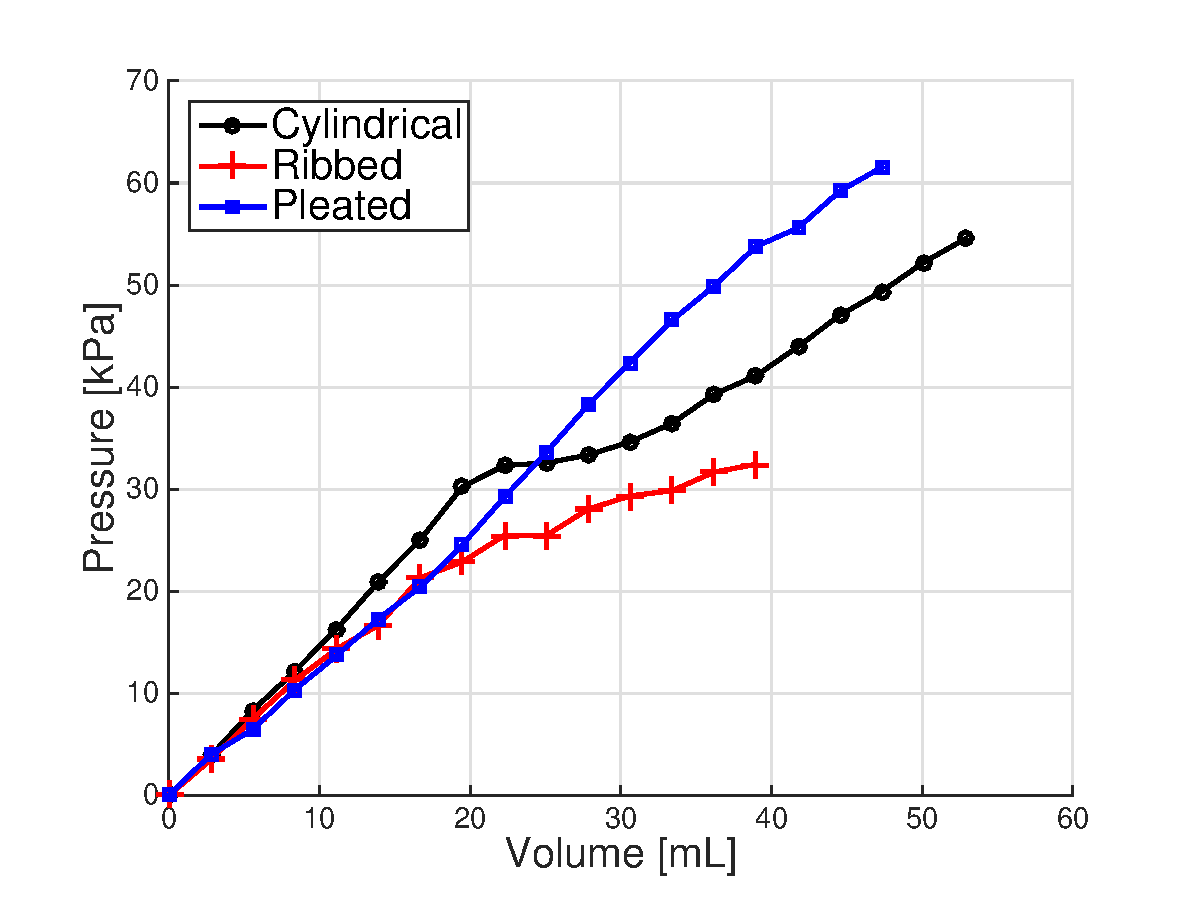
\includegraphics[width=0.95\columnwidth]{figures/actuators/morphologiescharacterization/PressureVsVolumeColor.eps}
            \caption{}
            \label{fig:Characterization_PressureVsVolume}
        \end{subfigure}
        \begin{subfigure}[b]{0.95\columnwidth}
            \centering
            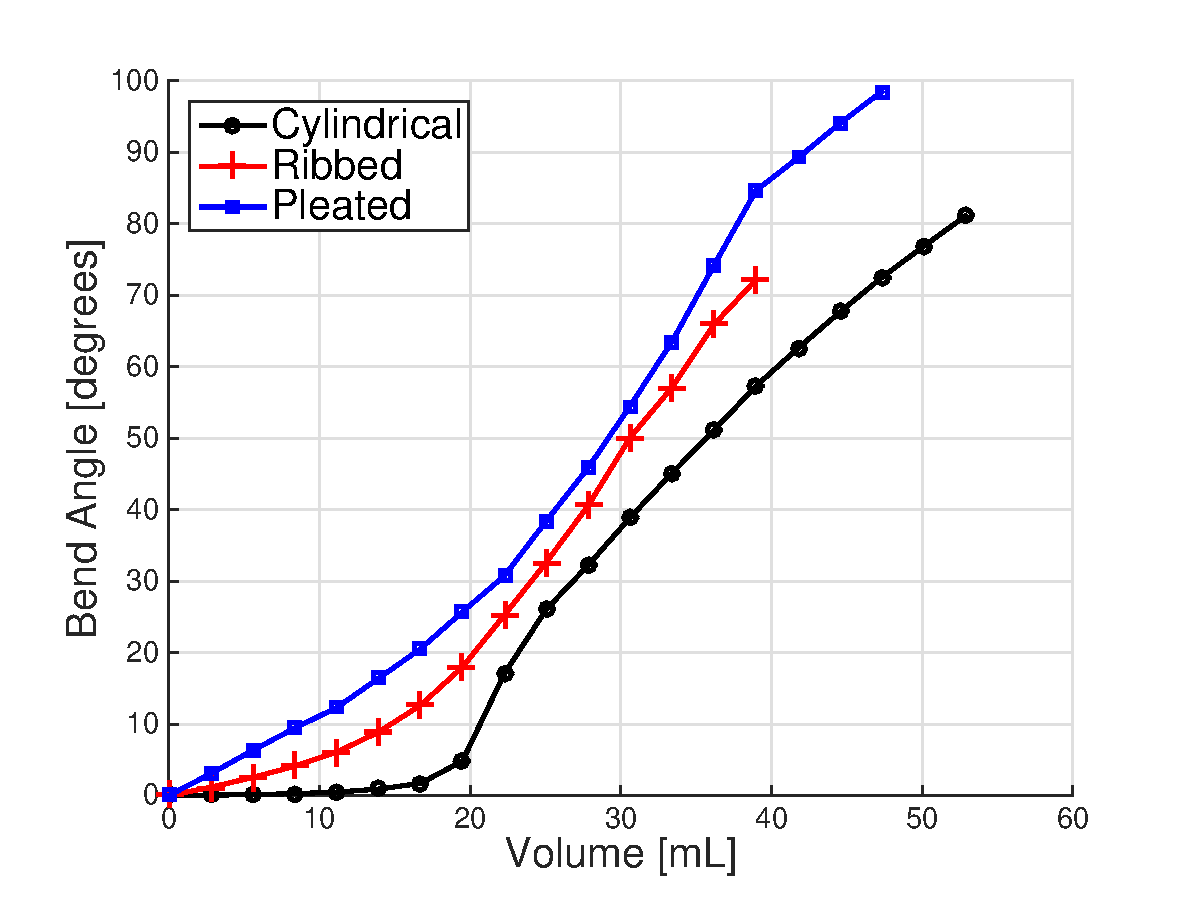
\includegraphics[width=0.95\columnwidth]{figures/actuators/morphologiescharacterization/BendAngleVsVolumeColor.eps}
            \caption{}
            \label{fig:Characterization_CurvatureVsVolume}
        \end{subfigure} \\
        \begin{subfigure}[b]{0.95\columnwidth}
            \centering
            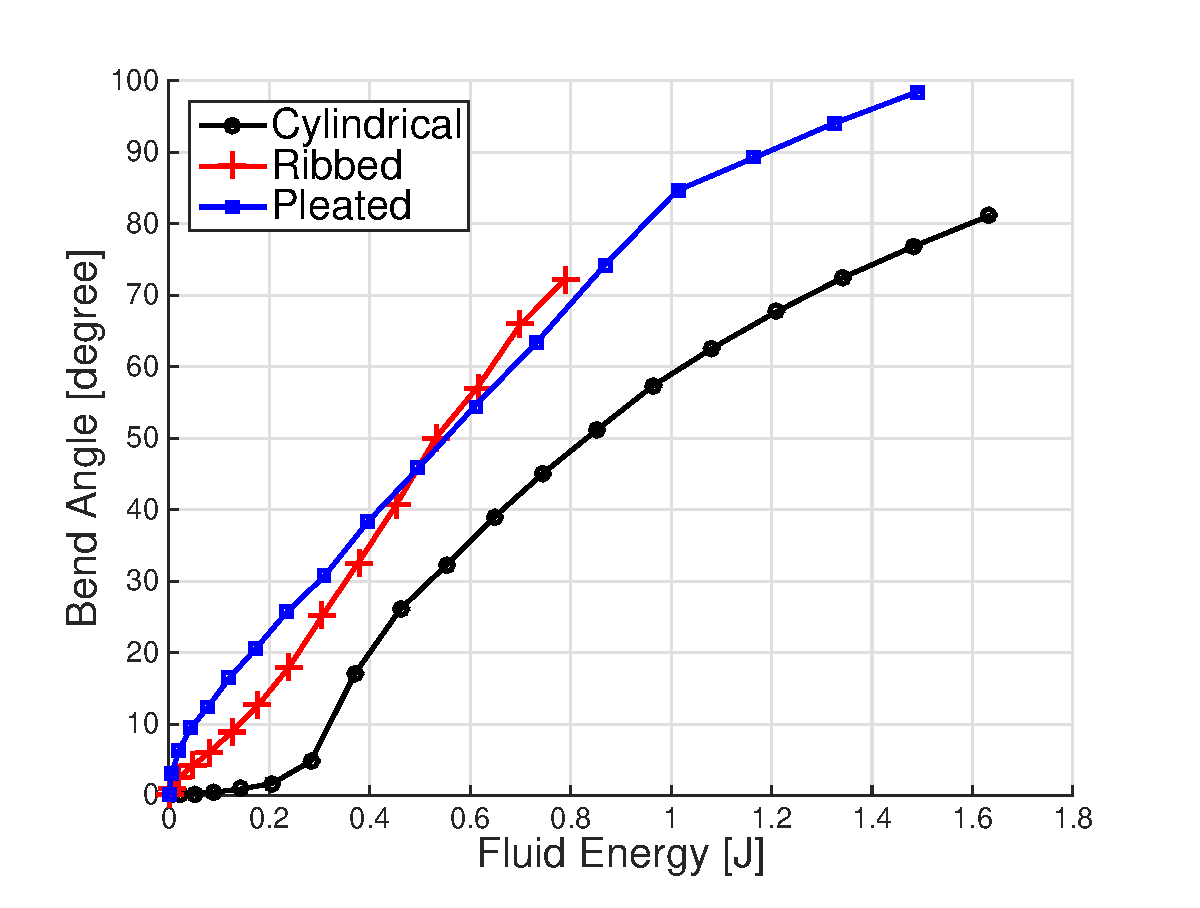
\includegraphics[width=0.95\columnwidth]{figures/actuators/morphologiescharacterization/BendAngleVsEnergyColor.eps}
            \caption{}
            \label{fig:Characterization_CurvatureVsEnergy}
        \end{subfigure}
        \begin{subfigure}[b]{0.95\columnwidth}
            \centering
            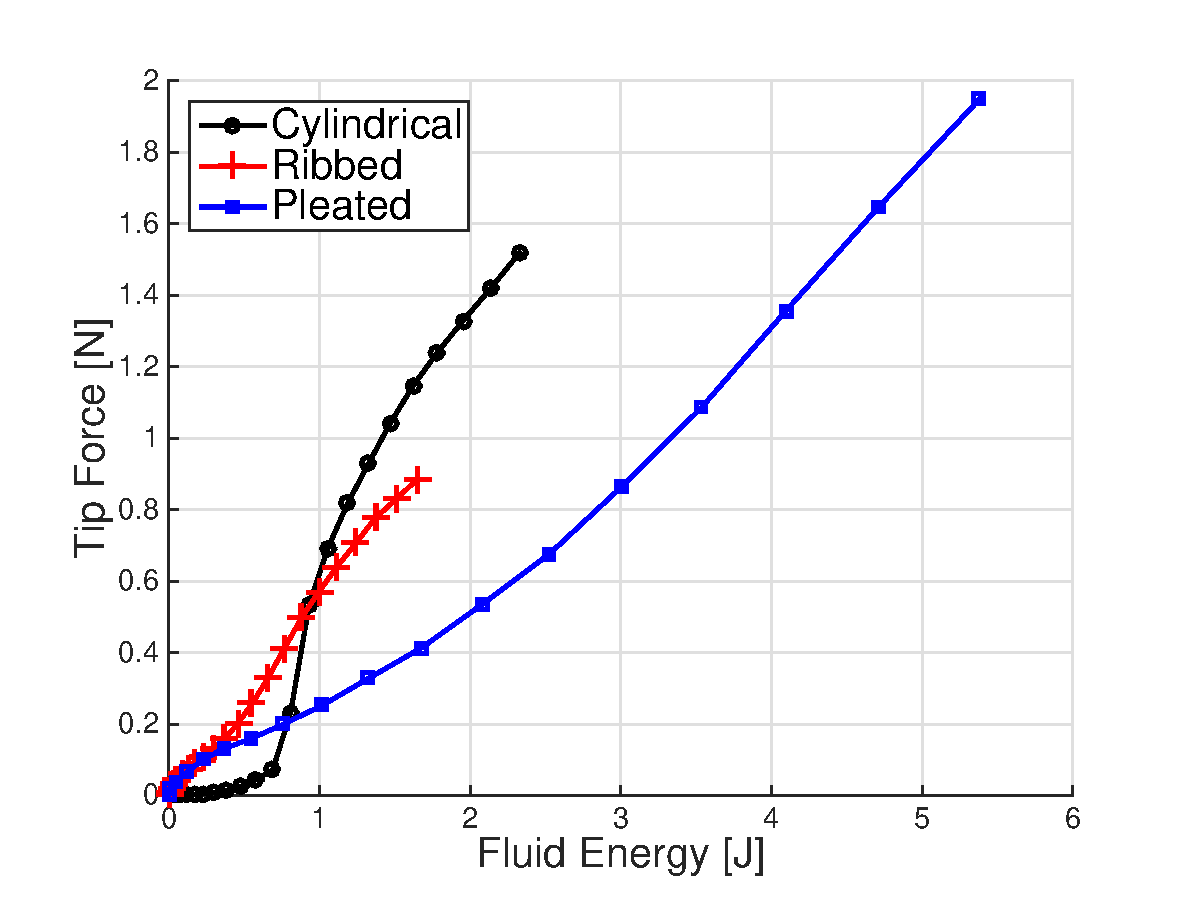
\includegraphics[width=0.95\columnwidth]{figures/actuators/morphologiescharacterization/ForceVsEnergyColor.eps}
            \caption{}
            \label{fig:Characterization_ForceVsEnergy}
        \end{subfigure}
        \caption[Experimental characterizations of three actuated segment morphologies.]{Experimental characterizations of three actuated segment morphologies performed by filling each actuator by means of controlled volumetric displacements and measuring internal pressure, neutral axis bend angle under a constant-curvature assumption, and blocking force.}\label{fig:actuator_characterization}
\end{figure*}

Figure~\ref{fig:actuator_characterization} details the results of these characterization experiments from which we can make several observations.
%
First, the pleated morphology is generally the stiffest, followed by the cylindrical, and then the ribbed, where stiffness is defined as $\frac{\partial p_c}{\partial \mathbb{V}_c}$ in the regime where $\mathbb{V}_c$ is greater than 25 mL (Fig.~\ref{fig:Characterization_PressureVsVolume}).
%
Second, the cylindrical morphology has a salient bend angle nonlinearity (Fig.~\ref{fig:Characterization_CurvatureVsVolume}).
%
More specifically, small volumetric fluid changes of less than $15\,$mL provide little control authority over curvature; however, above $25\,$mL displacements, the control authority is strong and the curvature-volume relationship is approximately linear.
%
Third, the cylindrical morphology requires the most amount of fluid energy to produce a given bend angle and the ribbed and pleated segments require approximately the same amount of fluid energy to generate equivalent bending (Fig.~\ref{fig:Characterization_CurvatureVsEnergy}).
%
Lastly, the pleated segment generally requires more fluid energy than both the ribbed and cylindrical morphologies to produce a given tip force.
%
However, the pleated segment can accommodate significantly higher input energies and therefore can reach the highest maximum tip force.
%



\section{Fabrication}
\label{sec:Fabrication}
Three distinct fabrication techniques for soft actuators are show-cased with the help of the previously described multi-segment arm designs.
Table~\ref{tab:MachineTools} contains the superscript references to machine tools and materials used.

	
\subsection{Lamination Casting with Heterogenous Embeddings}
\label{subsec:Fabrication, Lamination Casting with Heterogenous Embeddings}
lamination-based casting with heterogeneous embeddings is a fabrication technique that extends current soft lithography casting processes.
%
As detailed in Section~\ref{subsec:RW Fabrication} and in Figure~\ref{fig:RW fabrication}, the outer layers of a soft robot are often cast separately using soft lithography techniques to inlay channel structures. Then, these layers are laminated together with a constraint layer to form the actuator.
%
To power actuation, supply lines are pierced through the actuator's side wall and run external to the mechanism.
%
This approach can be prohibitive in that it creates an unreliable pneumatic interface between supply lines and actuated channels and also these external supply lines can inhibit the robot's movement or otherwise obstruct it from completing its intended function.
%
By embedding heterogeneous components within the elastomer layers as they are cast, we address both of these challenges.
%
In this section, we show how the idea of soft lithography can be combined with embedding heterogenous components and that it is well-suited for realizing the ribbed body segment morphology.
%
Specifically, we illustrate this fabrication process in the context of creating both a soft ribbed manipulator and soft ribbed fish robot.

A ribbed manipulator, like that detailed in Section~\ref{subsec:Manipulators, Ribbed}, can be fabricated using lamination-based casting with heterogeneous embeddings.
%
The specific approach for fabricating a six segment manipulator is illustrated in Figure~\ref{fig:ribbed fab process}.
Here, seven constraint supports (Fig.~\ref{fig:ribbed fab process}d) are 3D printed$^1$ and placed into a constraint layer mold (Fig.~\ref{fig:ribbed fab process}f), which is also 3D printed.
The constraint film (Fig.~\ref{fig:ribbed fab process}c) is cut from a thin acetal sheet$^8$ using a laser$^2$ and inserted through the aforementioned supports.
Above and below the constraint film, eight pieces of silicone tubing (Fig.~\ref{fig:ribbed fab process}a) are threaded through the supports.
Silicone rubber$^3$ is then mixed and poured into the constraint layer mold, immersing tubing, film, and supports in a layer of elastomer to create the composite constraint layer (Fig.~\ref{fig:ribbed fab process}g).
The uncured rubber inside the mold is then immediately degassed using a vacuum chamber$^4$.
Once cured, small holes are created in the constraint layer to pierce the embedded tubing at specific locations, allowing each line to independently address a group of fluidic channels.
Elastomer pieces containing channels (Fig.~\ref{fig:ribbed fab process}b) are casted and cured separately using a similar molding technique.
Those cured elastomer pieces (Fig.~\ref{fig:ribbed fab process}b) are then carefully attached to both faces of the constraint layer using a thin layer of silicone rubber.
Lastly, the printed feet (Fig.~\ref{fig:ribbed fab process}e) are attached to the constraint supports (Fig.~\ref{fig:ribbed fab process}d) to create an attachment point for ball transfers (Fig.~\ref{fig:ribbed_manipulator_design}d).
These mechanisms help constrain the arm's motion to a plane.
\begin{figure}[htb]
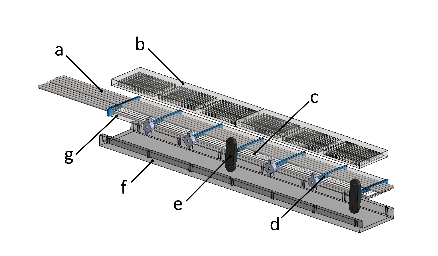
\includegraphics[width=\columnwidth]{figures/fabrication/fab_ribbed_process.eps}
\caption[Fabrication process for a ribbed manipulator morphology]{Fabrication process for a ribbed manipulator: silicone tubing (a), elastomer pieces containing channels (b), constraint film (c), constraint supports (d), feet (e), constraint layer mold (f), and composite constraint layer (g).}
\label{fig:ribbed fab process}
\end{figure}

The anatomically proportioned body of a fish-like robot developed by the authors in \citet{marchese2014autonomous} and detailed in Section~\ref{subsec:Locomotion, Pneumatic Fish} was also fabricated using a similar lamination-based casting process, and this process is detailed in Figure~\ref{fig:ribbed fab process_fish}.
Supply lines that connect the posterior actuator pair are embedded within the body during step 2 (Fig.~\ref{fig:ribbed fab process_fish}-2).
\begin{figure}[htb]
\includegraphics[width=\columnwidth]{figures/fabrication/fab_ribbed_process_fish.eps}
\caption{Illustration of the soft fish body fabrication process. First, two halves of the body (\textbf{1a}), a connector piece (\textbf{1b}), and a constraining layer (\textbf{1c}) are all cast from silicone using two-part molds. Next, these four pieces are sequentially bonded together using a thin layer of silicone (\textbf{2}). Lastly, once cured the fish body is ready for operation (\textbf{3}). This figure and caption are reproduced with permission from \citet{marchese2014autonomous}.}
\label{fig:ribbed fab process_fish}
\end{figure}

\subsection{Retractable Pin Casting}
\label{subsec:Fabrication, Retractable Pin Casting}
Retractable pin casting allows the relatively simple channel structure of the cylindrical body segment to be cast without lamination.
%
This fabrication process is advantageous because it eliminates the rupture-prone seems between the channels and constraint layer seem in the ribbed morphology fabricated through lamination-based casting.
%
Additionally, retractable pin casting is well-suited for the modular fabrication of multi-body soft robots.
%
Here, segments are individually cast and then concatenated together to form the robot.
%
Specifically, in this section we demonstrate retractable pin casting in the context of fabricating a cylindrical manipular.


A cylindrical manipulator, like that detailed in Section~\ref{subsec:Manipulators, Cylindrical}, is fabricated through a retractable-pin casting using pourable silicone rubber$^{3,5}$ and 3D printed molds$^1$.
Figure~\ref{fig:cylindrical_fab} details this process.
First, each body segment is independently fabricated in steps 1-3 and later these segments are joined serially to form the arm in steps 4 and 5.
To start, a four piece mold is printed.
The mold is then poured in two steps.
In step 1, a low elastic modulus rubber$^3$ is mixed, degassed in a vacuum$^4$, and poured to form the body segment's soft outer layer shown in \emph{white}.
The mold's outer piece, one half of it is shown in \emph{green}, functions to form the segment's exterior.
Metal rods shown in \emph{pink} are inserted into the mold and are held in place by the \emph{orange} bottom piece of the mold.
These rods will form the cavities for the segment's two lateral fluidic actuation channels.
After the outer layer has cured, the \emph{red} rigid sleeve is removed in step 2 from the extruded feature of the \emph{orange} bottom piece of the mold.
This produces a cavity into which a slightly stiffer rubber$^5$ is poured, forming the segment's partially constraining inner layer shown in \emph{cyan}.
The extruded feature of the \emph{orange} bottom piece, shown by its \emph{orange} end tip, functions to produce the segment's hollow interior core.
In step 3, the body segments are removed from their molds and joined to rubber$^5$ endplates shown in \emph{cyan} using silicone adhesive$^6$.
The small \emph{yellow} channel inlets were added on one side of the \emph{pink} metal pins during step 1.
In step 4, soft silicone tubes$^7$ are joined to each embedded channel's inlet.
The resulting bundle of tubes is passed through each segment's hollow interior.
Lastly, in step 5 multiple body segments are attached at their endplates using the same adhesive$^6$.

\begin{figure}[htb]
\centering
\includegraphics[width=\columnwidth]{figures/fabrication/fab_cylindrical_process.eps}
\caption[Fabrication process for the cylindrical manipulator morphology]{Fabrication process for the cylindrical manipulator morphology: Each body segment is casted using a two step process where the outer soft layer (\textbf{1}) and inner stiffer layer (\textbf{2}) are poured. Once cured, the segments are joined to endplates using silicone adhesive (\textbf{3}). Next, silicone tubing is connected to each embedded channel and the resulting tubing bundle is run inside each segment's hollow interior (\textbf{4}). Lastly, the body segments are serially connected using adhesive to form the manipulator (\textbf{5}).}
\label{fig:cylindrical_fab}
\end{figure}

\subsection{Lost Wax Casting}
\label{subsec:Fabrication, Lost Wax Casting}
As mentioned, existing soft robots are often produced through a multi-step lamination process, which produces seams and is prone to delamination.
By abandoning the need for lamination, the retractable pin fabrication process enables seamless channel structures; however, the channel structures are limited to a relatively simple shape.
%
For these reasons, we introduce lost-wax casting as part of the fabrication process for soft actuators.
%
With this, arbitrarily shaped internal channels can be achieved to enable a wider range of applications.
%
As examples, in this section we fabricate a pleated uni-directional gripper and a ribbed soft fish tail using the lost-wax approach.

The complete fabrication process for a pleated actuator consists of eight steps that are depicted in Figure~\ref{fig:pleated_fab}.
\begin{figure*}[htb]
\centering
   \includegraphics[width=2\columnwidth]{figures/fabrication/fab_pleated_process_horizontal.eps}
      \caption[Fabrication process for the pleated actuator morphology]{Fabrication process for the pleated actuator morphology: (\textbf{A}) Pour and cure a rubber mold, (\textbf{B}) pour wax core with embedded supportive rod, (\textbf{C}) combine bottom mold, top mold and wax core using pins, (\textbf{D}) pour rubber into assembled mold, (\textbf{E}) pour stiffer rubber on top of the cured actuator to form a constraint layer, (\textbf{F}) remove cured actuator from mold, (\textbf{G}) melt out wax core from the actuator using an oven, and (\textbf{H}) add silicone tubing and plug using silicone sealant.}
      \label{fig:pleated_fab}
\end{figure*}
In step (A), harder silicone rubber$^{10}$ is poured into a mold, which contains a 3D printed model of the wax core.
In preparation for step (B), the model is removed and the rubber mold is left inside the outer mold.
Next, a rigid rod or tube, for example made of carbon fiber$^{12}$, is used as a supportive inlay for the wax core.
The rod is laid into the cavity of the rubber mold, supported on both ends by the outer mold.
This ensures that the wax core does not break when removed from the rubber mold.
Mold release spray is applied to the silicone rubber mold to ease the wax core removal process.
The wax$^{11}$ is heated up until it becomes fully liquefied.
The assembly of the rubber mold and the outer mold is heated up for a few minutes to the same temperature as the wax.
Using a syringe, the liquid wax is injected into the assembly.
Within a few minutes, the injected wax will start to solidify and significantly shrink in volume; this is counteracted by injecting more hot wax into the solidifying wax core during the cool down period.
In step (B), the wax core is first allowed to completely cool down, then it is released from the mold.
In step (C), the cooled down wax core is assembled together with the bottom mold, which defines the pleated structure of the actuator.
The mold assembly is aligned with a top mold using pins. This top mold provides additional volume to cover the wax core.
In step (D), low elastic modulus rubber$^3$ is mixed, degassed in a vacuum$^4$, and poured to form the pleats and allowed to cure.
In step (E), stiffer rubber is poured on top of the cured pleats to form a constraint layer.
In step (F), the cured actuator is removed from the mold.
In step (G), most of the wax core is melted out by placing the cured actuator into an oven in an upright position.
After this, remaining wax residues are cooked out in a boiling water bath.
Finally, in step (H) a silicone tube$^9$ and a piece of silicone cord$^13$ get covered with silicone adhesive$^6$ and are inserted into the front and back holes, respectively.
The actuator can be used as a unidirectional gripper (see Figure~\ref{fig:cylindrical_design}) or as one agonist actuated segment within a multiple body manipulator (see Section~\ref{subsec:Manipulators, Pleated}).

The actuated body of the hydraulic fish detailed in Section~\ref{subsec:Locomotion, Hydraulic Fish} is also produced via lost-wax casting. The fabrication process is depicted in Figure~\ref{fig:fabrication}.
\begin{figure}[htb]
        \centering
         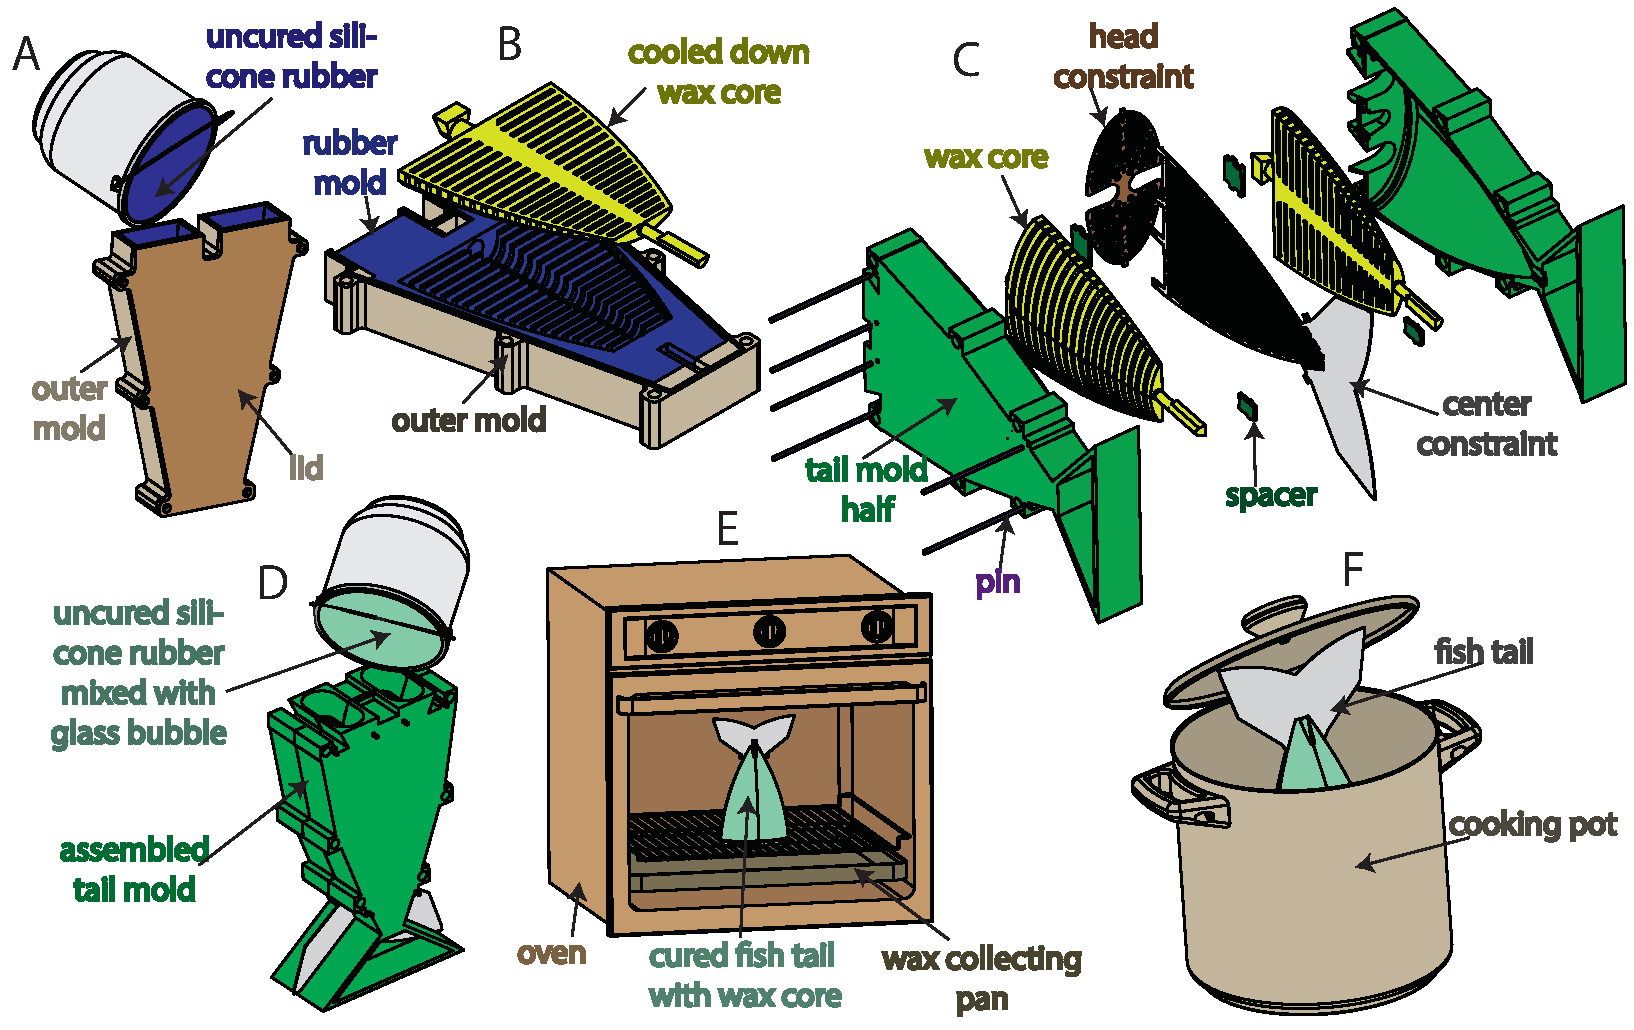
\includegraphics[width=0.99\columnwidth]{figures/fabrication/fab_hydraulic_fish_tail.pdf}
         \caption[Fish tail fabrication process]{Fish tail fabrication process: (\textbf{A}) Pour and cure a rubber mold, (\textbf{B}) pour wax cores, (\textbf{C}) combine head constraint, center constraint and wax cores with tail mold halves, (\textbf{D}) pour rubber mixed with glass bubbles into assembled tail mold, (\textbf{E}) using an oven melt out wax core from the cured fish tail, and (\textbf{F}) cook out remaining wax to create desired actuator cavities.}\label{fig:fabrication}
\end{figure}
In step (A), the rubber mold is poured and cured inside an assembly consisting of an outer mold with lid and a model for the core inside of it.
In preparation for step (B), the lid and the model core are removed and the rubber mold is left inside the outer mold.
The rubber mold receives a small carbon fiber tube as an inlay in its center cavity.
This ensures that the wax core does not break when being removed from the rubber mold.
Mold release spray is applied to the silicone rubber mold to ease the wax core removal process.
The wax is heated up until it becomes fully liquefied.
The assembly of rubber mold and outer mold is heated up for a few minutes to the same temperature as the wax.
Using a syringe, the liquid wax is injected into the assembly.
Within a few minutes, the injected wax will start to solidify and significantly shrink in volume; this is counteracted by injecting more hot wax into the solidifying wax core during the cool down.
In step (B), the wax core is first allowed to completely cool down, then it is released from the mold.
In step (C), a head constraint, a center constraint, and two wax cores are assembled together inside the tail mold halves using spacers, positioning pins and screws.
In step (D), a mix of silicone rubber with glass bubbles is poured into the tail assembly and allowed to cure.
In step (E), most of the wax core is melted out by placing the fish tail in an upright position into an oven. Finally, in step (F) the remaining wax residues are cooked out in a boiling water bath.

\begin{table}[htb]
\caption{Commercially Available Tools and Equipment}
\centering
\begin{tabular}{c l l}
\hline
\hline
\# & Product Name & Company\\
\hline
1 & Fortus 400mc & Stratasys\\
2 & VLS3.50 & Universal Laser Systems\\
3 & Ecoflex 0030 & Smooth-On\\
4 & AL Cube & Abbess Instr. \& Systems\\
5 & Mold Star 15 & Smooth-On\\
6 & Silicone Sealant 732 & Dow Corning\\
7 & PN 51845K52 & McMaster\\
8 & PN 5742T51 & McMaster\\
9 & PN 51845K53 & McMaster\\
10 & Mold Star 30 & Smooth-On\\
11 & Beeswax & Jacquard\\
12 & PN 2153T31& McMaster\\
13 & PN 9808K21& McMaster\\
\hline
\end{tabular}
\label{tab:MachineTools}
\end{table} 

\section{Power}
\label{sec:Power}
The objective of the power system is to provide real-time adjustment of fluid energy input to the manipulators.

%The power system is used in conjunction with the curvature controllers developed in Section~\ref{sec:Control} and the kinematic algorithms developed in Section~\ref{sec:Kinematic Modeling} to achieve closed-loop configuration control of the manipulators.

In general, fluid power can be achieved by controlling either pressure or volume.
We choose volume control because it offers the ability to: (i) measure the control variable via linear displacement as opposed to pressure transducers, (ii) set a maximum safe displacement limit, and (iii) vary pre-pressurization of segments to accommodate for differences in actuator compliance.

\subsection{Fluidic Drive Cylinder}
\label{subsec:Power, FDC}
In order to independently and bidirectionally actuate arm segments, an array of custom fluidic drive cylinders were developed.
These cylinders provide fluidic power to the arm by producing volumetric changes within a segment's embedded channels.
Linear actuators are directly coupled to and control the positional displacements of the pistons within fluidic cylinders.
Accordingly, these linear actuators govern the volumetric displacement of fluid out of the cylinders and into a segment's embedded channels, and vice versa.
Figure~\ref{fig:DriveCylinderOverview} illustrates the components of a fluidic drive cylinder.
\begin{figure}[thb]
\centering
   \includegraphics[width=\columnwidth]{Figures/power/DriveCylinderOverview.eps}
   \caption[An overview of the fluidic drive cylinders.]{An overview of two fluidic drive cylinders used to drive the curvature of a bi-directional arm segment. (a) An electric linear actuator$^5$ is directly attached to the piston of a fluidic cylinder$^6$ (c) via a 3D-printed coupler (b). Fluid is displaced through the inlet (e) and outlet (d) of the cylinder. A motor controller$^7$ (f) allows digital command signals to govern fluid movement.}
   \label{fig:DriveCylinderOverview}
\end{figure}

\subsection{Fluidic Drive Cylinder Model}
\label{subsec:Power, Model}
In the following, a model of the fluidic drive cylinder is developed.
Although this plant model is not used in the control of the cylinder, it serves to identify the impact design decisions have on the system's input-output relationships.
Figure~\ref{fig:CylinderModel} shows a simplified schematic representation of the closed-loop fluidic power delivery system.
A linear time-invariant dynamic model can be created to \emph{approximate} the behavior of a fluidic drive cylinder connect to an elastomer channel, and we refer to this as the plant in Figure~\ref{fig:CylinderModel}.

In order to develop the plant model, we make the following assumptions:
\begin{enumerate}
  \item The motor has no inductance. We justify this by observing that the dynamics of the electrical system are considerably faster than the dynamics of the fluidic system.
  \item The piston moves without friction inside the cylinder. We justify this by observing that most of the plant's energy is removed via the highly resistive fluid transmission line between the cylinder and channel.
  \item The channel's compliance $C_c$, which is the ratio of its change in volume to change in pressure, is piecewise constant with respect to channel pressure.
  \item The fluid's compliance $C_f$, which is also the ratio of its change in volume to change in pressure, is constant with respect to fluid pressure. This is, because linearizing the ideal gas law around the operating point $p_0$ at constant temperature $T_0$ leads to $\mathbb{V} = -\frac{m R T_0}{p_0^2} \, p = C_f \, p$.
  \item The fluid's mass is negligible, because we are currently only working with gases, specifically air.
\end{enumerate}

\begin{figure}[htb]
\centering
   \includegraphics[width=\columnwidth]{Figures/power/CylinderModel}
   \caption[Parameters used in developing a simplified fluidic drive cylinder model.]{Parameters used in developing a simplified fluidic drive cylinder model. A schematic representation of the plant shows a linear electric actuator (left), a piston and fluidic cylinder (middle), and an elastomeric channel grouping within an arm segment (right). A PID controller runs the plant with the volumetric displacement as its reference value, the motor voltage as its control effort and the sensed volumetric displacement as its feedback.}
   \label{fig:CylinderModel}
\end{figure}

The equations of motion for the drive cylinder are expressed in the following. First, the piston's linear motion can be approximated as
\begin{equation}\label{eq:eom1}
    F_m - p_s \, A_p \approx \frac{m_p}{A_p} \ddot{\mathbb{V}}_s,
\end{equation}
where $F_m$ is the force exerted by the linear motor on the piston, $p_s$ is the gauge pressure of the fluid inside the cylinder, $A_p$ is the cross sectional area of the piston, $m_p$ is the mass of the piston, and $\mathbb{V}_s$ is the volumetric displacement of the cylinder.
We can derive the next equation of motion by observing that the total volume of fluid within the plant (represented as the dotted area in Fig.~\ref{fig:CylinderModel}), does not change as this is a closed-circuit drive system.
It follows that $\Delta \, \mathbb{V} \approx 0$ and therefore
\begin{equation}\label{eq:eom2}
    \dot{\mathbb{V}}_s + \dot{p}_s \, C_f + \dot{p}_c \, \left( C_f + C_c \right) \approx 0.
\end{equation}
Here, $p_c$ is the gauge pressure of the fluid within the elastomer channel and $C_f$ and $C_c$ are the compliances of the transmission fluid and elastomer channel, respectively. The volumetric fluid flow into the cylinder is approximated as
\begin{equation}\label{eq:eom3}
    \dot{\mathbb{V}}_s + \frac{p_c - p_s}{R_t} \approx -C_f \dot{p}_s,
\end{equation}
where $R_t$ is the resistance of the fluid transmission line connecting the cylinder and channel. Lastly, the force output of the linear actuator can be approximated as
\begin{equation}\label{eq:eom4}
    F_m \approx - \frac{\beta \, \lambda}{R_m \, A_p} \, \dot{\mathbb{V}}_s + \frac{\beta}{R_m} \, e_m.
\end{equation}
Above, $\beta$ is the motor constant relating motor current to the force of the linear actuator. The motor constant $\lambda$ relates linear velocity to the counter EMF voltage, $R_m$ is the motor's resistance, and $e_m$ is the input motor voltage.

Using these equations of motion, a SISO LTI open-loop plant model can be expressed in the form
$\dot{\mathbf{x}} = \mathbf{A}_{\text{OL}}\,\mathbf{x} + \mathbf{B}_{\text{OL}}\, u$ and
$y = \mathbf{C}_{\text{OL}}\,\mathbf{x}$,
and is explicitly written in Equation~\ref{eq:LTI}.
Combining Equation~\ref{eq:eom1} and \ref{eq:eom4} yields the first row.
The second row is found by combining Equation~\ref{eq:eom2} and \ref{eq:eom3}, and the third row is Equation~\ref{eq:eom3}.

\footnotesize
\begin{align}\label{eq:LTI}
\nonumber  \begin{bmatrix}
  \ddot{\mathbb{V}}_s \\
  \dot{p}_c \\
  \dot{p}_s
  \end{bmatrix} &=
  \setlength{\arraycolsep}{2pt}
  \begin{bmatrix}
  -\frac{\beta \lambda}{m_p R_m} & 0 & -\frac{A_p^2}{m_p} \\
  0 & \frac{1}{\left( C_f + C_c \right) R_t} & -\frac{1}{\left( C_f + C_c \right) R_t} \\
  -\frac{1}{C_f} & -\frac{1}{C_f R_t} & \frac{1}{C_f R_t}
  \end{bmatrix}
  \begin{bmatrix}
  \dot{\mathbb{V}}_s \\
  p_c \\
  p_s
  \end{bmatrix} +
  \begin{bmatrix}
  \frac{\beta A_p}{m_p R_m} \\
  0 \\
  0
  \end{bmatrix} e_{m}\\
  y &=
  \begin{bmatrix} 0 & 1 & 0
  \end{bmatrix}
  \begin{bmatrix}
  \dot{\mathbb{V}}_s \\
  p_c \\
  p_s
  \end{bmatrix}
\end{align}
\normalsize

For bounded-input, bounded-output stability, it is sufficient to use a proportional control law taking the form
\begin{equation}
    e_m(t) = K_p \, \left( \mathbb{V}_r(t) - \mathbb{V}_s(t) \right),
\end{equation}
where $\mathbb{V}_r$ is a reference volume and $K_p$ is a proportional gain constant. However, to ensure zero steady-state error in tracking the reference volume and for a suitable dynamic response, we implement a traditional PID control law
\begin{eqnarray}
    e_m(t) = K_p \,\mathbb{V}_{e}(t) + K_i \, \int_0^t \mathbb{V}_{e}(\tau) \text{d}\tau + K_d \, \frac{\text{d} \mathbb{V}_{e}(t)}{\text{d} t}\\
    \mathbb{V}_{e}(t) = \mathbb{V}_r(t) - \mathbb{V}_s(t).
\end{eqnarray}

Approximations of the model's parameters are listed in Table \ref{tab:ModelParameters}. We approximate the transmission line resistance as
\begin{equation}
    R_t \approx \frac{128 \, \mu \, L_t}{\pi \, d_t^4},
\end{equation}
where $\mu$ is the fluid's viscosity, $L_t$ is the transmission line's length, and $d_t$ is the transmission line's inside diameter.
Figure~\ref{fig:compliancePlot} details the experimentally determined pressure-volume relationship of both the transmission fluid and the compliant elastomer channel.
Channel compliance was determined by actuating a fluidic elastomer actuator with an incompressible fluid and measuring the resulting internal pressuring while incrementally increasing channel volume.
The incompressible fluid enables channel compliance to be decoupled from transmission fluid compliance.
By linearizing this experimental data, the fluid compliance $C_f$ and the piecewise defined channel compliance $C_{c1}$ and $C_{c2}$ can be determined. Also the linearization offset $\mathbb{V}_{\text{off}}$ can be found.
To verify the plant model, model predicted transmission line flow $\frac{p_s - p_c}{R_t}$ was compared to experimentally measured flow (Fig.~\ref{fig:flowVerification}).
To obtain flow data, a flow transducer was placed inline with the transmission tubing.
\begin{figure}[htb]
\centering
   \includegraphics[width=\columnwidth]{Figures/power/compliancePlot_new.eps}
   \caption[Experimentally measured actuator compliance]{Experimentally measured pressure-to-volume relationship of air $(C_f)$ and of air and elastomer channel combined $(C_f + C_c)$.}
   \label{fig:compliancePlot}
\end{figure}

\begin{figure}[htb]
\centering
   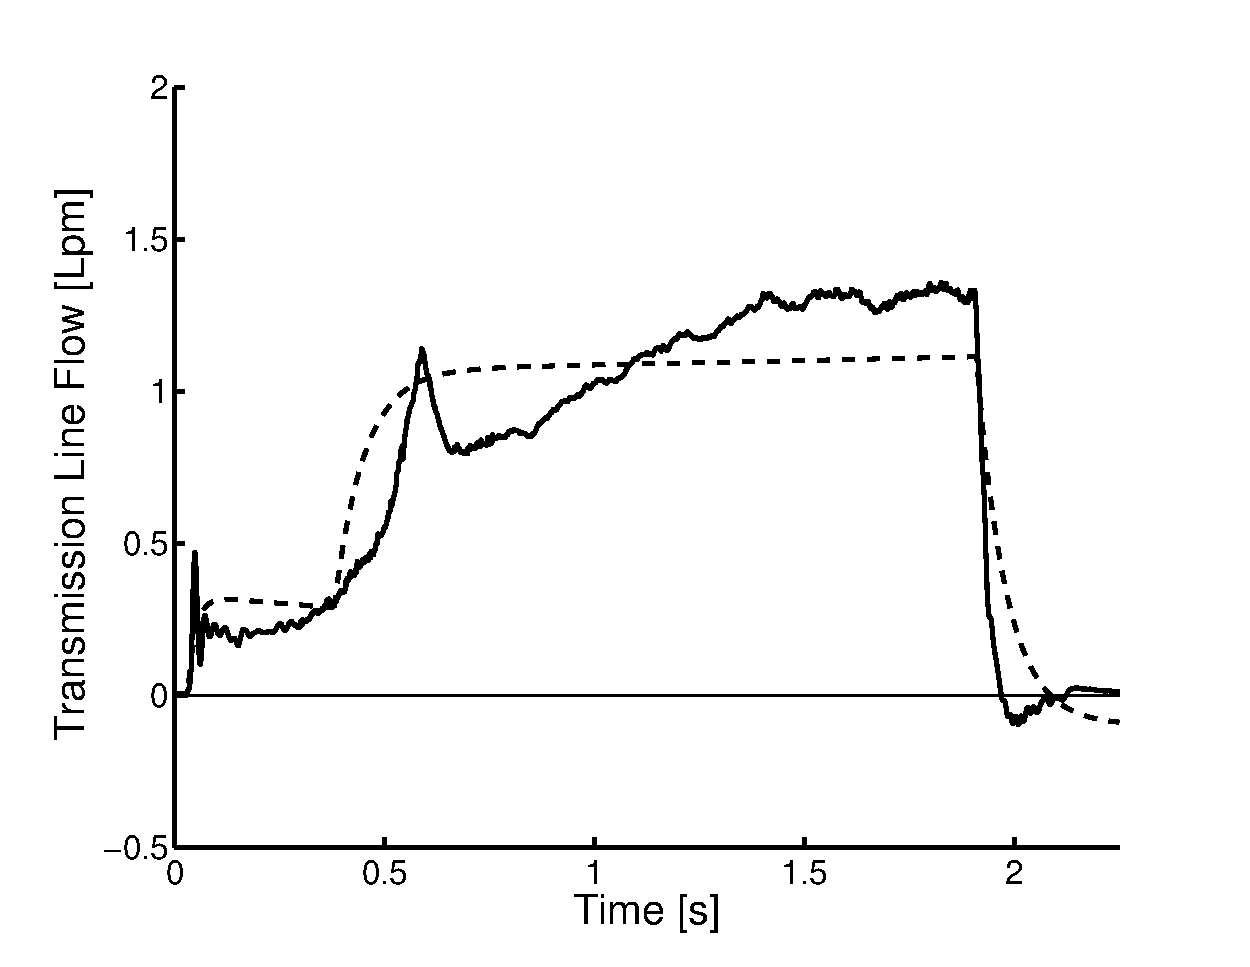
\includegraphics[width=\columnwidth]{Figures/power/flowVerification.eps}
   \caption[Experimental verification of the fluidic drive cylinder plant model.]{Experimental verification of the fluidic drive cylinder plant model. The solid line represents measured transmission line flow, and the dotted line represents model predicted flow.}
   \label{fig:flowVerification}
\end{figure}

\begin{table}[htb]
\centering
\footnotesize
\tabcolsep=0.11cm
\begin{tabular}{c c c c c c c c c c}
\hline\hline
$\beta$ & $\lambda$ & $m_{p}$ & $R_{m}$ & $A_{p}$ & $C_{f}$ & $C_{c1}$ & $C_{c2}$ & $V_{\text{off}}$ & $R_{t}$ \\
232 & 475 & 0.19 & 18.5 & 7.92 & -2.0e-10 & 1.25e-10 & 4.15e-9 & -9.3e-05 & 3.4e8\\
$\frac{\text{N}}{\text{A}}$ & $\frac{\text{V}\text{ s}}{\text{m}}$  & kg & $\Omega$ & \text{cm}$^2$ & $\frac{\text{m}^3}{\text{Pa}}$ & $\frac{\text{m}^3}{\text{Pa}}$ & $\frac{\text{m}^3}{\text{Pa}}$& $\text{m}^3$ & $\frac{\text{Pa s}}{\text{m}^3}$\\[1ex]
\hline
\end{tabular}
\caption{Approximations of fluidic drive cylinder parameters}
\label{tab:ModelParameters}
\end{table}
%C_f = -8.756e-6/4.378e4 = -2.0000e-10
%C_c1 = -8.437e-6/2.661e4 - C_f = 1.1706e-10
%C_c2 = (1.833e-5 - 9.186e-6)/(3.447e4-2.806e4) - C_f = 1.2265e-09
%V_off = 9.186e-6 - (2e-10+1.2265e-9)*2.806e4 = -3.0842e-05

\subsection{Fluidic Drive Cylinder Implementation}
\label{subsec:Power, Implementation}
Fluidic drive cylinders are mechanisms, which interface the computational and algorithmic aspects of the manipulation system with the soft arm.
Specifically, they input digital command signals from a control algorithm and generate fluidic pressure that drives the curvature of the arm segments.

Two drive cylinders are used to control a single bidirectional segment.
Although the mapping of either the agonistic or antagonistic channel deformation is monotonically related to a single piston's displacement, when considering bidirectional segment movement as well as positive and negative curvatures, the two drive cylinders must be controlled synchronously.
One piston is held still and the other piston is moved in either forward or reverse to increase or decrease curvature. There are four distinct states of a pair of fluidic drive cylinders in this arrangement as detailed in Figure~\ref{fig:DriveCylinderStates}.
%First, if the curvature is negative and the error in curvature (red arc - blue arc) is positive, then the cylinder driving the left channel grouping is driven in reverse (top left). Second, if the curvature is positive and the error in curvature is negative, then the right cylinder is driven in reverse (top right). Third, if the curvature is positive and the error positive, the right cylinder is driven forward (bottom left). And lastly, when curvature is negative and the error is negative, the left cylinder is driven forward (bottom right).
\begin{figure}[thb]
\centering
   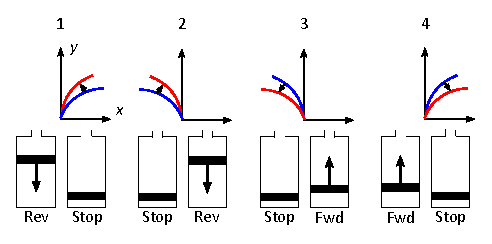
\includegraphics[width=\columnwidth]{Figures/power/DriveCylinderStates.eps}
   \caption[Diagram depicting the driving states of the fluidic drive cylinders]{Diagram depicting the four driving states of the two fluidic drive cylinders used to control an arm segment. These states depend on the error in curvature (measured state shown as blue arcs minus target state shown as red arcs) as well as the sign of the curvature (right hand rule). (\textbf{1}) The curvature is negative and the error is positive. (\textbf{2}) The curvature is positive and the error is negative. (\textbf{3}) The curvature is positive and the error is positive. (\textbf{4}) The curvature is negative and the error is negative.}
   \label{fig:DriveCylinderStates}
\end{figure} 

\section{Locomotion}
\label{sec:Locomotion}
Soft and continuously deformable locomotion systems can be made from fluidic elastomer body segments.
Specifically, in this section we detail how soft robotic fish can be composed by combining the actuated segments that were presented in Section~\ref{subsec:Actuators, Actuator Morphologies} with a portable power system.

\subsection{Pneumatic Fish}
\label{subsec:Locomotion, Pneumatic Fish}
The soft pneumatic fish developed in \cite{marchese2014autonomous} with a ribbed actuator is shown as a complete system in Figure~\ref{fig:pneumaticfish_system} and performing an escape response in Figure~\ref{fig:pneumaticfish_escape}.

\begin{figure}[htb]
        \centering
        \begin{subfigure}[b]{\columnwidth}
            \centering
            \includegraphics[width=0.9\columnwidth]{Figures/locomotion/pneumaticfish_system.png}
            \caption{}
            \label{fig:pneumaticfish_system}
        \end{subfigure}\\
        \begin{subfigure}[b]{\columnwidth}
            \centering
            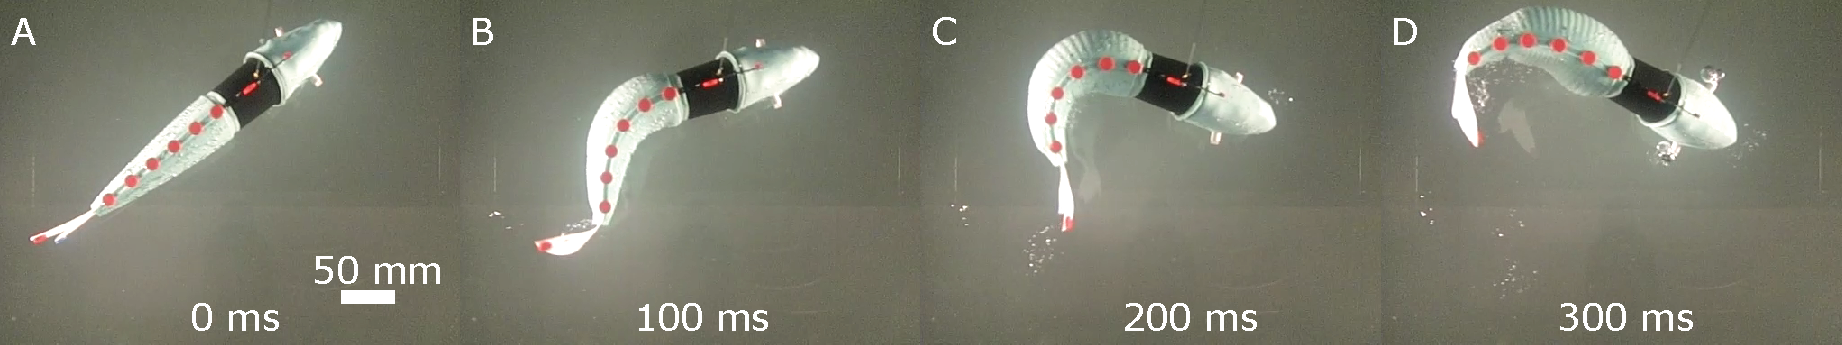
\includegraphics[width=0.9\columnwidth]{Figures/locomotion/pneumaticfish_escape_half.pdf}
            \caption{}
            \label{fig:pneumaticfish_escape}
        \end{subfigure}%
        \caption[Pneumatic Fish.]{A soft pneumatic robotic fish: (\textbf{a}) An overview of the robotic system, photo courtesy of Devon Jarvis, (\textbf{b}) A sequence depicting the fish performing an escape response.}
\end{figure}



\subsection{Hydraulic Fish}
\label{subsec:Locomotion, Hydraulic Fish}
The soft hydraulic fish~\cite{katzschmann2014hydraulic} with a single ribbed actuator is shown as a complete system in Figure~\ref{fig:hydraulic_fish_system_overview}. A close-up view is shown in Figure~\ref{fig:hydraulic_fish_yaw} and the 3d swimming capabilities are shown in Figure~\ref{fig:hydraulic_fish_all_motions}.

\begin{figure}[htb]
        \centering
        \begin{subfigure}[b]{0.48\columnwidth}
            \centering
           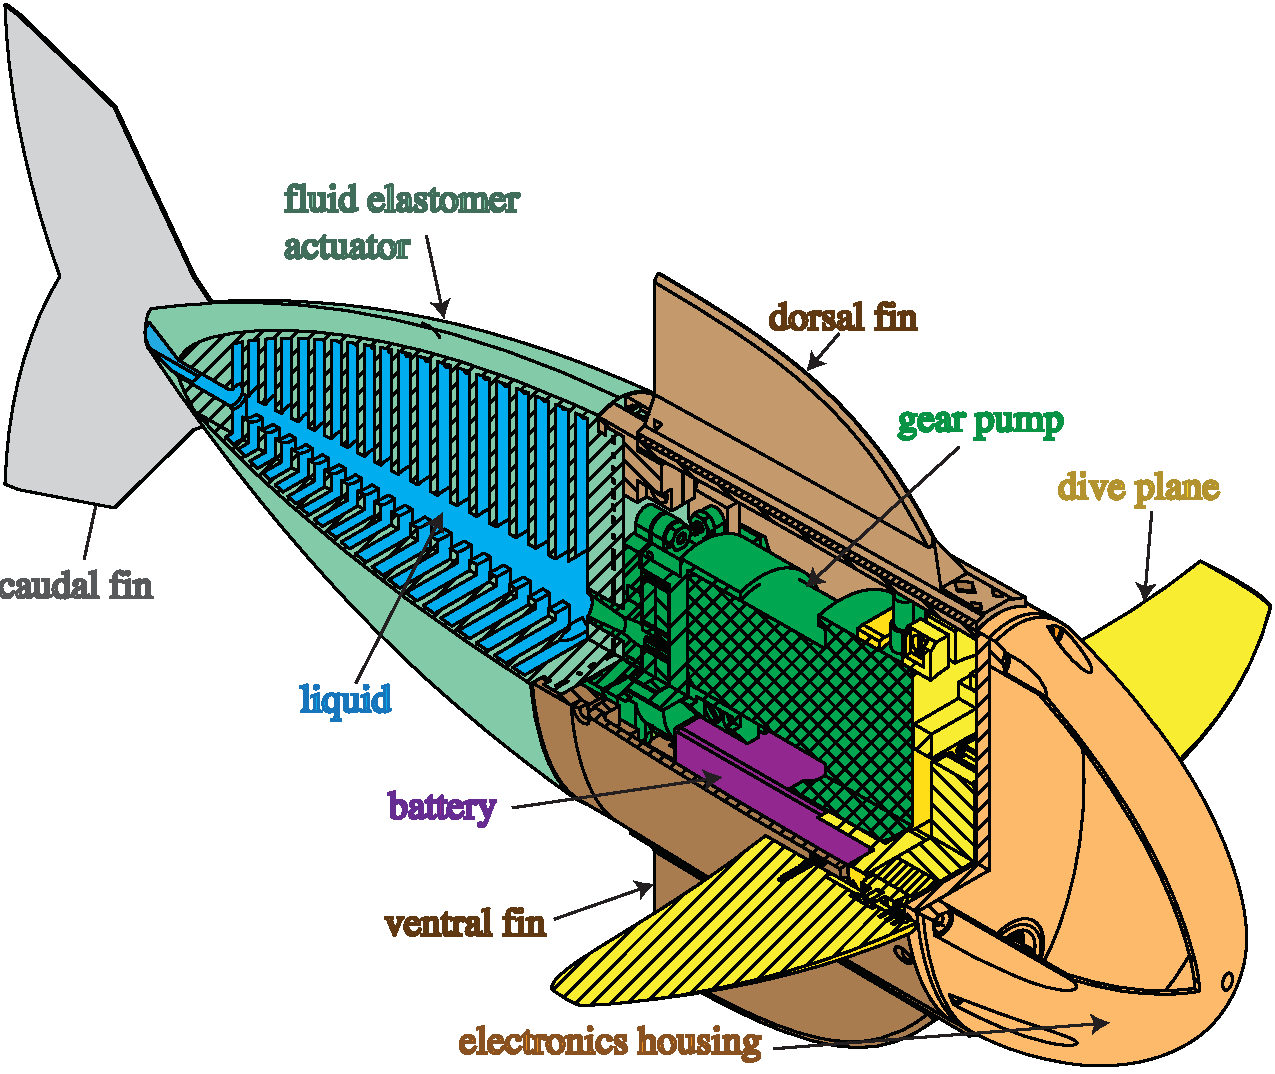
\includegraphics[width=1\columnwidth]{figures/locomotion/hydraulic_fish_system_overview.pdf}
           \caption{}
            \label{fig:hydraulic_fish_system_overview}
        \end{subfigure}
        \begin{subfigure}[b]{0.48\columnwidth}
            \centering
            \includegraphics[width=1\columnwidth]{figures/locomotion/hydraulic_fish_yaw.png}
            \caption{}
            \label{fig:hydraulic_fish_yaw}
        \end{subfigure}\\
        \begin{subfigure}[b]{1\columnwidth}
            \centering
            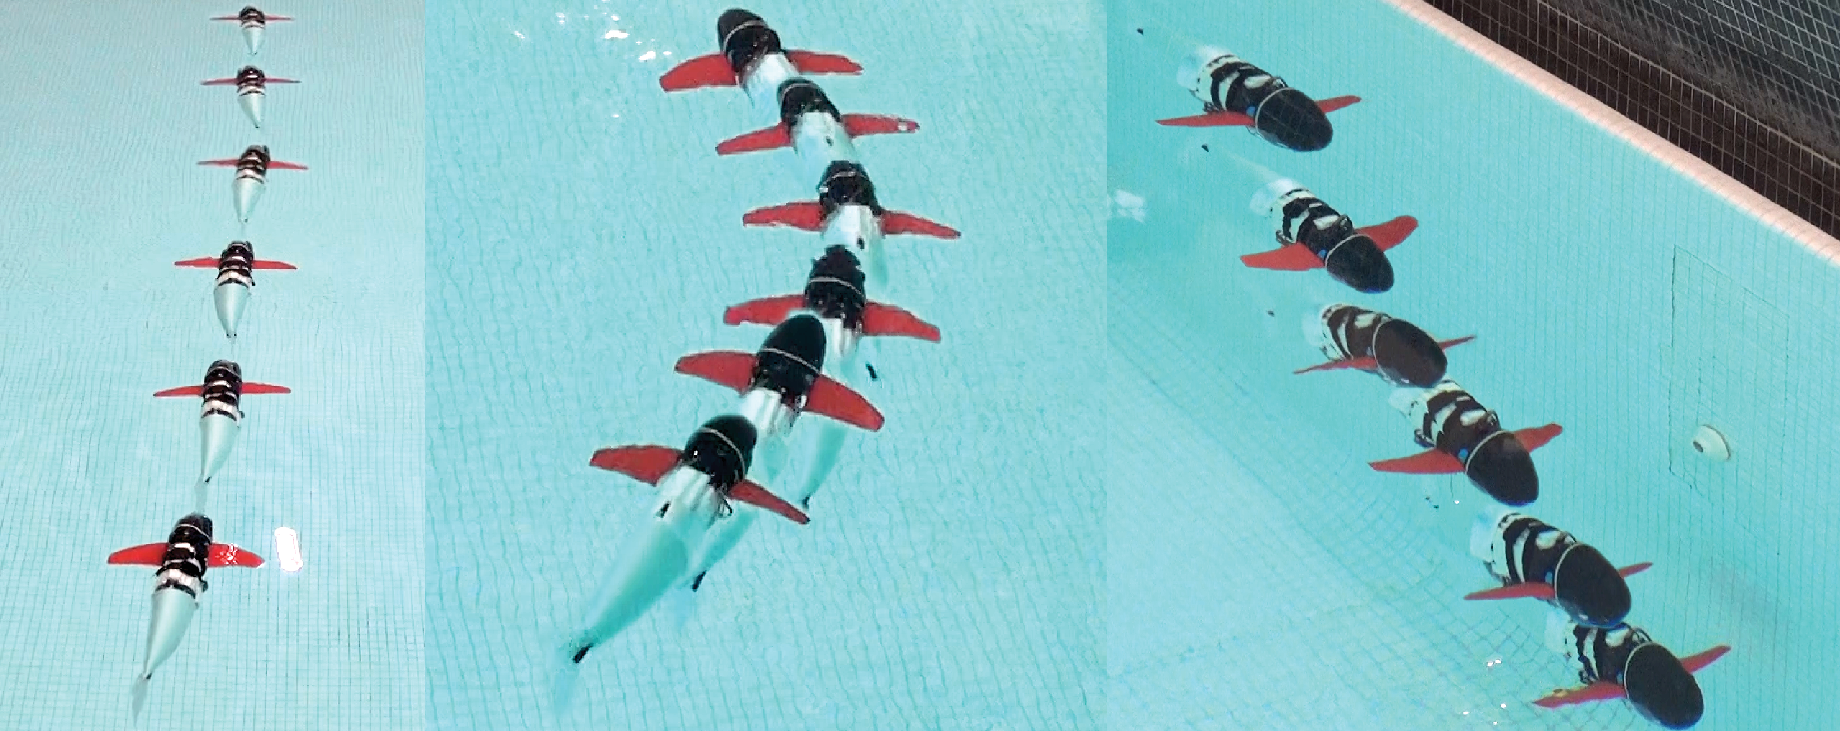
\includegraphics[width=1\columnwidth]{figures/locomotion/hydraulic_fish_all_motions.pdf}
            \caption{}
            \label{fig:hydraulic_fish_all_motions}
        \end{subfigure}%
        \caption[Hydraulic soft robotic fish]{A soft hydraulic robotic fish: (\textbf{a}) A schematic of the system, (\textbf{b}) underwater swimming motion, and (\textbf{c}) example of continuous forward swimming, yaw motion, and diving.}
\end{figure} 

\section{Manipulators}
\label{sec:Manipulators}
Soft and continuously deformable manipulators can be assembled from bending fluidic elastomer segments.
Specifically, in this section we detail how multi-segment manipulators can be composed by serially concatenating the actuated segments that were presented in Section~\ref{subsec:Actuators, Actuator Morphologies}.

\subsection{Ribbed}
\label{subsec:Manipulators, Ribbed}
Structurally, a ribbed arm is composed of serially concatenated, homogeneous ribbed body segments.
In this work, the manipulator's reachable envelope is constrained to the x-y plane.
%, as shown in Section~\ref{sec:System Overview}.
By volume, over ninety-seven percent of the ribbed manipulator is soft silicone rubber, excluding the feet.
This manipulator is depicted in Figure~\ref{fig:ribbed_manipulator_design} and can theoretically be composed of any number of the aforementioned ribbed segments (Fig.~\ref{fig:ribbed_manipulator_design}e).
Practically, we have constructed a six-segment prototype (Fig. \ref{fig:ribbed_manipulator_real}).
All twelve fluidic transmission lines as well as channel-to-supply interfaces are embedded within the manipulator's center layer.
Markers are located at the interface between segments (Fig.~\ref{fig:ribbed_manipulator_design}b), making segment endpoints identifiable to an external localization system.
The starting point of the arm's first segment (Fig.~\ref{fig:ribbed_manipulator_design}a) is grounded to the platform on which the arm moves and we refer to this as the base.
Ball transfers (Fig.~\ref{fig:ribbed_manipulator_design}d) are also located at each segment endpoint to allow the arm to move on a two-dimensional plane with minimal friction.
In many experiments conducted throughout this work, the pose of the arm's end-effector (Fig.~\ref{fig:ribbed_manipulator_design}c) is controlled.

\begin{figure}[htb]
        \centering
        \begin{subfigure}[b]{\columnwidth}
            \centering
            \includegraphics[width=0.9\columnwidth]{figures/manipulators/ribbed_manipulator}
            \caption{}
            \label{fig:ribbed_manipulator_design}
        \end{subfigure}\\
        \begin{subfigure}[b]{\columnwidth}
            \centering
            \includegraphics[width=0.9\columnwidth]{figures/manipulators/ribbed_manipulator_real}
            \caption{}
            \label{fig:ribbed_manipulator_real}
        \end{subfigure}%
        \caption[A ribbed soft manipulator prototype.]{A ribbed soft manipulator prototype. (\textbf{a}) The arm is composed of homogeneous and independently actuated ribbed segments (e). The base of the arm's first segment is fixed (a) and the end of its last segment is the end-effector (c). Markers (b) identify the endpoints of each segment and ball transfers (d) mitigate friction. (\textbf{b}) Photographs of the ribbed manipulator prototype.}
\end{figure}

\subsection{Cylindrical}
\label{subsec:Manipulators, Cylindrical}
We can also compose a manipulator from cylindrical fluidic elastomer segments, as shown in Figure~\ref{fig:cylindrical_manipulator}.
Just as in the ribbed composition, cylindrical segments are joined end-to-end.
Here, fluid transmission lines are passed through the manipulator's hollow center.
This feature not only facilitates segment concatenation, but also allows for modular composition of a manipulator, because transmission lines are not permanently embedded within the elastomer.
Additionally, this manipulator type is only composed of soft silicone rubber as there is no inextensible constraint.
No other materials are used, except for the attached ball transfers to mitigate ground friction.
\begin{figure}[htb]
\centering
\includegraphics[width=\columnwidth]{Figures/manipulators/cylindrical_manipulator_real}
\caption[A cylindrical soft manipulator prototype.]{A cylindrical soft manipulator prototype with and without a pleated finger-like gripper.} \label{fig:cylindrical_manipulator}
\end{figure}

\subsection{Pleated}
\label{subsec:Manipulators, Pleated}
A manipulator can also be composed from pleated fluidic elastomer segments, as shown in Figure~\ref{fig:pleated_manipulator}.
Just as in the ribbed and cylindrical composition, pleated segments are joined end-to-end.
The fluid transmission lines are passed through along the central axis of the segments.
A supportive hollow profile can be added to combine two segments.
This pleated design allows for modular composition of a manipulator, because transmission lines are not permanently embedded within the elastomer.
Additionally, this type of manipulator is, like the cylindrical manipulator, composed entirely of soft silicone rubber.

\begin{figure}[htb]
\centering
\includegraphics[width=\columnwidth]{Figures/manipulators/pleated_manipulator_real}
\caption[A pleated soft manipulator prototype.]{A pleated soft manipulator prototype, composed of two segments with two degrees of freedom each.}
\label{fig:pleated_manipulator}
\end{figure} 

%\input{capabilities}
%\clearpage

%\input{experimental_results}
%\clearpage

\section{Discussion}
\label{sec:discussion}
% What did we achieve?
The design of the actuators and fabrication methods described in this paper provide recipes for the rapid fabrication of modular soft robots with arbitrary body morphology.
%
%New capabilities
This class of soft robots is very well-suited for tasks requiring: (i) interactions with humans and environments to be safe, (ii) uncertainty to be mitigated at the hardware level, (iii) continuous and dexterous deformation, and/or (iv) hardware to take an unstructured, amorphous form.
%
For example, by making robots from soft elastic materials, with no sharp edges, and with relatively low link inertia, a robot's reliance on sensors and software for safety is reduced.
%
The prospects for safe integrations between a robot and human are generally increased when the compliance of the material composing the machine match those of soft biological materials \citet{majidi2014soft}, and this feature is inherent to robots made of soft silicone elastomer.
%
An alternative approach is to allow resilient soft machines to handle some uncertainty at the hardware level in order to reduce the burden on the computational system.
%
For example, consider how a soft manipulator passively conforms to the environment's boundary. The planner is unaware of this complex interaction, but the primary task can still be successfully executed.
%
Further, modern inspection tasks as well as invasive surgery require devices with redundant degrees of freedom and high dexterity and often impose the constraint of navigating around sensitive objects.
%
As initially demonstrated here, soft robotic manipulators may be well-suited for this class of tasks.

%What are the limitations and open problems



%Lastly, this work brings to attention the need for proprioceptive localization systems for soft robots. Feedback for our controller comes currently from an exteroceptive localization system. This is a reasonable method for indoor, laboratory or factory environments where there is sufficient line of sight to the manipulator. However, this sensor approach is prohibitive in that the environment must be equipped with cameras and the tasks cannot occlude the view of these cameras onto the manipulator. Proprioceptive localization for soft robots is an important avenue for future research.


\section*{Acknowledgments}
\label{sec:Acknowledgments}
This work was done in the Distributed Robotics Laboratory at MIT with support from the National Science Foundation, grant numbers NSF 1117178, NSF EAGER 1133224, NSF IIS1226883, and NSF CCF1138967 as well as NSF Graduate Research Fellowship Program, primary award number 1122374. We are grateful for this support. The authors declare no competing financial interests. Photo in Figure~\ref{fig:intro_new}c courtesy of Devon Jarvis for Popular Mechanics. 

\bibliography{main}

\end{document}
